
\chapter{Finite Element Method}

Ciarlet's definition of a finite element is:

\begin{definition}[Finite element] A finite element is a triple $(T, V_{T}, \Psi_{T})$, where
\begin{enumerate}
\item $T$ is a bounded set
\item $V_{T}$ is function space on $T$ of finite dimension $N_T$ 
\item $\Psi_{T} = \{ \psi^1_T, \ldots , \psi^{N_T}_T \}$ is a set of linearly independent functionals on $V_{T}$.
\end{enumerate}
\end{definition}

\noindent
The nodal basis $\{\varphi^1_T\, \ldots \varphi^{N_T}_T\}$ for $V_T$ is the basis 
dual to $\Psi_T$, i.e., 
$$
\psi^i_T (\varphi^j_T) = \delta_{ij}
$$
Barycentric coordinates are useful to express the nodal basis functions.


Finite elements with point evaluation functionals are called Lagrange  
finite elements, elements using also derivatives are called Hermite finite elements.

Usual function spaces on $T \subset \setR^2$ are
\begin{eqnarray*}
P^p & := & \mbox{span} \{ x^i y^j : 0 \leq i, \, 0 \leq j, \, i+j \leq p \} \\
Q^p & := & \mbox{span} \{ x^i y^j : 0 \leq i \leq p, \, 0 \leq j \leq p  \}
\end{eqnarray*}

Examples for finite elements are
\begin{itemize}
\item A linear line segment 
\item A quadratic line segment
\item A Hermite line segment
\item A constant triangle
\item A linear triangle
\item A non-conforming triangle
\item A Morley triangle
\item A Raviart-Thomas triangle
\end{itemize}
The local nodal interpolation operator defined for functions $v \in C^m(\overline T)$ is
$$
I_T v := \sum_{\alpha = 1}^{N_T} \psi^\alpha_T(v) \varphi^\alpha_T
$$
It is a projection.


Two finite elements $(T,V_T, \Psi_T)$ and 
$(\widehat T, V_{\widehat T}, \Psi_{\widehat T})$ are called 
{\em equivalent} if there exists an invertible function $F$ such that
\begin{itemize}
\item $T = F (\widehat T)$
\item $V_T = \{ \hat v \circ F^{-1} : \hat v \in V_{\widehat T} \}$
% \item $\Psi_T = \{ \psi_{\widehat T} (. \circ F) \}$
\item $\Psi_T = \{ \psi^T_i : V_T \rightarrow \setR : v \rightarrow \psi^{\hat T}_i (v \circ F) \}$
\end{itemize}
Two elements are called affine equivalent, if $F$ is an affine-linear function.

Lagrangian finite elements defined above are equivalent. The Hermite elements are not equivalent.

Two finite elements are called interpolation equivalent if there holds
$$
I_T (v) \circ F = I_{\widehat T} (v \circ F)
$$

\begin{lemma} Equivalent elements are interpolation equivalent
\end{lemma}

The Hermite elements define above are also interpolation equivalent.

A regular triangulation ${\cal T} = \{ T_1, \ldots, T_M \}$ of a domain 
$\Omega$ is the subdivision of a domain $\Omega$ into closed triangles $T_i$
such that $\overline \Omega = \cup T_i$ and $T_i \cap T_j$ is 
\begin{itemize}
\item either empty
\item or an common edge of $T_i$ and $T_j$
\item or $T_i = T_j$ in the case $i = j$.
\end{itemize}
%
In a wider sense, a triangulation may consist of different element shapes such
as segments, triangles,  quadrilaterals, tetrahedra, hexhedra, prisms, pyramids.


A finite element complex $\{ (T, V_T, \Psi_T) \}$ is a set of finite elements
defined on the geometric elements of the triangulation ${\cal T}$.

It is convenient to construct finite element complexes such that all
its finite elements are affine equivalent to one {\em reference finite element} $(\widehat T, \hat V_T, \hat \Psi_T)$. The transformation $F_T$ is such that
$T = F_T (\widehat T)$.


Examples: linear reference line segment on $(0,1)$.


The finite element complex allows the definition of the global 
interpolation operator for $C^m$-smooth functions by
$$
I_{\cal T} v_{|T} = I_T v_T \qquad \forall \, T \in {\cal T}
$$
%
The finite element space is 
$$
V_{\cal T} := \{ v = I_{\cal T} w : w \in C^m(\overline \Omega) \}
$$

We say that $V_{\cal T}$ has regularity $r$ if $V_{\cal T} \subset C^r$.
If $V_{\cal T} \neq C^0$, the regularity is defined as~$-1$.

Examples:
\begin{itemize}
\item
The $P^1$ - triangle with vertex nodes leads to regularity $0$.
\item
The $P^1$ - triangle with edge midpoint nodes leads to regularity $-1$.
\item
The $P^0$ - triangle leads to regularity $-1$.
\end{itemize}

\medskip

For smooth functions, functionals $\psi_{T,\alpha}$ and $\psi_{\widetilde T, \tilde \alpha}$ sitting in the same location are equivalent. The set of global 
functionals $\Psi  = \{ \psi_1, \ldots, \psi_N\}$ is the linearly independent
set of functionals containing all (equivalence classes of) local functionals.

The connectivity matrix $C_T \in \setR^{N \times N_T}$ is defined such
that the local functionals are derived from the global ones by
$$
\Psi_T (u) = C_T^t \Psi (u)
$$
Examples in 1D and 2D


The nodal basis for the global finite element space is the
basis in $V_{\cal T}$ dual to the global functionals $\psi_j$, i.e., 
$$
\psi_j(\varphi_i) = \delta_{ij}
$$
There holds
\begin{eqnarray*}
\varphi_i|_T & = & 
I_T \varphi_i = \sum_{\alpha = 1}^{N_T} \psi_T^\alpha (\varphi_i) \varphi^\alpha_T \\
& = & \sum_{\alpha = 1}^{N_T} (C_T^t \psi(\varphi_i))_\alpha \varphi_T^\alpha \\
& = & \sum_{\alpha = 1}^{N_T} (C_T^t e_i)_\alpha \varphi_T^\alpha = \sum_{\alpha = 1}^{N_T} C_{T,i\alpha} \varphi_T^\alpha 
\end{eqnarray*}


\section{Finite element system assembling}

As a first step, we assume there are no Dirichlet boundary conditions.
The finite element problem is
\begin{equation}
\label{equ_femproblem}
\mbox{Find } u_h \in V_{\cal T} \mbox{ such that } : A (u_h, v_h) = f(v_h) \qquad \forall \, v_h \in V_{\cal T}
\end{equation}
The nodal basis and the dual functionals provides the one to one relation 
between $\setR^N$ and $V_{\cal T}$:
$$
\setR^N \ni \underline u \leftrightarrow u_h \in V_{\cal T} \qquad \mbox{with} \qquad 
u_h = \sum_{i=1}^N \varphi_i \underline u_i \qquad \mbox{and} \qquad
\underline u_i = \psi_i (u_h).
$$
Using the nodal basis expansion of $u_h$ in (\ref{equ_femproblem}), and
testing only with the set of basis functions, one has

$$
A( \sum_{i=1}^N u_i \varphi_i, \varphi_j) = f(\varphi_j) \qquad \forall \, j = 1 \ldots N
$$
With
$$
A_{ji} = A(\varphi_i, \varphi_j) \qquad \mbox{and} \qquad \underline f_j = f(\varphi_j),
$$
one obtains the linear system of equations
$$
A \underline u = \underline f
$$
The preferred way to compute the matrix $A$ and vector $f$ is a sum over element 
contributions. The restrictions of the bilinear and linear form to the elements are
$$
A_T(u,v) = \int_T \nabla u \cdot \nabla v \, dx + 
        \int_{\partial \Omega \cap T} \alpha u v \, ds
$$
and
$$
f_T(v) = \int_T f v \, dx + 
        \int_{\partial \Omega \cap T} g v \, ds
$$
Then 
$$
A(u,v) = \sum_{T \in \cal T} A_T(u,v)  \qquad
f(v) = \sum_{T \in \cal T} f_T(v)
$$
On each element, one defines the $N_T \times N_T$ {\bf element matrix}  and 
{\bf element vector} in terms of the local basis on $T$:
$$
A_{T,\alpha \beta} = A_T (\varphi^T_\beta, \varphi^T_\alpha)
\qquad \qquad
\underline{f}_{T,\alpha} = \underline{f}_T (\varphi^T_\alpha)
$$

Then, the global matrix and the global vector are
$$
A = \sum_{T \in \cal T} C_T A_T C_T^t
$$
and
$$
\underline f = \sum_{T \in \cal T} C_T \underline f_T
$$


Namely,
\begin{eqnarray*}
\underline f_i & = & f(\varphi_i) = \sum_{T \in \cal T} f_T (\varphi_i|_T) = 
\sum_{T \in \cal T} f_T (\sum_\alpha C_{T,i\alpha} \varphi_T^\alpha) \\
& = &
\sum_{T \in \cal T} \sum_{\alpha} C_{T,i\alpha} f_T (\varphi_T^\alpha) =
\sum_{T \in \cal T}  \sum_{\alpha} C_{T,i\alpha} \underline f_\alpha
\end{eqnarray*}
and
\begin{eqnarray*}
A_{ji} & = & \sum_{T \in \cal T} A(\varphi_i|_T, \varphi_j|_T) = 
         \sum_{T \in \cal T} A (\sum_\alpha C_{T,i\alpha} \varphi_T^\alpha,
                                      \sum_\beta C_{T,j\beta} \varphi_T^\beta) \\
        & = & \sum_{T \in \cal T} \sum_\alpha \sum_\beta C_{T,i\alpha} A_{T,\alpha \beta} C_{T,j\beta}
\end{eqnarray*}

\bigskip

On the elements $T$, the integrands are smooth functions. Thus, numerical
integration rules can be applied.

\bigskip

In the case of Dirichlet boundary conditions,
let $\gamma_D \subset \{ 1, \ldots , N \}$ correspond to the vertices $x_i$
at the Dirichlet boundary, and $\gamma_f = \{ 1, \ldots N \} \setminus \gamma_D$.

We have the equations
$$
\sum_{i \in \gamma_D} A_{ji} u_i + \sum_{i \in \gamma_f} A_{ji} u_i = f_j
\qquad \forall \, j \in \gamma_f
$$
Inserting $u_i = u_D(x_D)$ for $i \in \gamma_i$ results in the reduced system
$$
\sum_{i \in \gamma_f} A_{ji} u_i = f_j - \sum_{i \in \gamma_D} A_{ji} u_D(x_i)
$$

An alternative approach is to approximate Dirichlet boundary conditions by
Robin b.c., $\frac{\partial u}{\partial n} + \alpha u = \alpha u_D$, with large 
parameter $\alpha$.

\section{Finite element error analysis}
%
Let $u$ be the solution of the variational problem, and $u_h$ its
Galerkin approximation in the finite element sub-space $V_h$. Cea's Lemma 
bounds the finite element error $u - u_h$ by the 
best approximation error 
$$
\| u - u_h \|_V \leq C \inf_{v_h \in V_h} \| u - v_h \|_V.
$$
The constant factor $C$ is the ratio of the continuity bound and the
coercivity bound of the bilinear form $A(.,.)$.

Provided that the solution $u$ is sufficiently smooth,
we can take the finite element interpolant to bound the best approximation 
error:
$$
\inf_{v \in V_h} \| u - v_h \|_V \leq \| u - I_{\cal T} u \|_V
$$
In the following, we will bound the interpolation error.


\begin{lemma} Let $\widehat T$ and $T$ be $d$-dimensional domains related
by the invertible affine linear transformation $F_T : \widehat T \rightarrow T $ 
$$
F_T (x) = a + B x,
$$
where $a \in \setR^d$ and $B$ is a regular matrix in $\setR^{d\times d}$.
Then there holds:
\begin{equation}
\| u \circ F_T \|_{L_2(\widehat T)} = (\det B)^{-1/2} \, \| u  \|_{L_2(T)}
\end{equation}
%
\begin{equation}
\frac{\partial}{\partial x_{i_m}} \ldots 
\frac{\partial}{\partial x_{i_1}} \left( u \circ F_T \right) = 
\sum_{j_m = 1}^d \ldots \sum_{j_1=1}^d 
\left(
\frac{\partial}{\partial x_{j_m}} \ldots 
\frac{\partial}{\partial x_{j_1}} u \right) \circ F_T \; \;
B_{j_m,i_m} \ldots B_{j_1, i_1}
\end{equation}
%
\begin{equation}
| u \circ F |_{H^m(\widehat T)} \leqc (\det B)^{-1/2} \| B \|^m  \, | u |_{H^m(T)}
\end{equation}
\end{lemma}

{\em Proof:} Transformation of integrals, chain rule. \hfill $\Box$


\bigskip
We define the diameter of the element $T$
$$
h_T = \operatorname{diam} T 
$$
A triangulation is called {\bf shape regular}, if all its elements fulfill
$$
| T | \geqc h_T^2
$$
with a ``good'' constant $\sim 1$. If one studies convergence, one considers families
of triangulations with decreasing element sizes $h_T$. In that case, the family
of triangulations is called shape regular, if there is a common constant $C$ such that 
all elements of all triangulations fulfill $| T | \geq C h_T^2$.


\begin{lemma} Let $F_T = a + B x$ be the mapping from the reference triangle
to the triangle $T$. Let $|T| \geqc h_T^2$. Then there holds
\begin{eqnarray*}
\| B_T \| & \eqc & h_T \\
\| B_T^{-1} \| & \eqc & h_T^{-1}
\end{eqnarray*}
\end{lemma}


The following lemma is the basis for the error estimate. This lemma is the main
application for the Bramble Hilbert lemma. Sometimes, it is called 
the Bramble Hilbert lemma itself:
\begin{lemma}
Let $(T, V_T, \Psi_T)$ be a finite element such that
the element space $V_T$ contains polynomials up to order $P^k$. 
Then there holds
$$
\| v - I_T v \|_{H^1} \leq C | v |_{H^m} \qquad \forall \, v \in H^m(T)
$$
for all $m > d/2$, $m \geq 1$, and $m \leq k+1$.
\end{lemma}
{\em Proof:} First, we prove that $id - I_T$ is a bounded operator
from $H^m$ to $H^1$:
\begin{eqnarray*}
\| v - I_T v \|_{H^1} & \leq & \| v \|_{H^1} + \| I_T v \|_{H^1}
        =  \| v \|_{H^1} + \| \sum_{\alpha} \psi_\alpha(v) \varphi_\alpha \|_{H^1}
 \\
& \leq & \| v \|_{H^1} + \sum_\alpha \| \varphi_\alpha \|_{H^1} | \psi_\alpha(v) | \\
& \leqc & \| v \|_{H^m}
\end{eqnarray*}
The last step used that for $H^m$, with $m > d/2$, point evaluation is continuous.
Now, let $v \in P^k(T)$. Since $P^k \subset V_T$, and $I_T$ is a projection on $V_T$, 
there holds $v - I_T v = 0$. The Bramble Hilbert Lemma applied for $U = H^1$ and
$L = id - I_T$ proves the result.
\hfill $\Box$



To bound the finite element interpolation error, we will transform
functions from the elements $T$ to the reference element $\widehat T$.

\begin{theorem} Let ${\cal T}$ be a shape regular triangulation of $\Omega$.
Let $V_{\cal T}$ be a $C^0$-regular finite element space such that all local spaces contain $P^1$. Then there holds
$$
\| v - I_{\cal T} v \|_{L_2(\Omega)} \leqc  \left\{ \sum_{T \in {\cal T}} h_T^4 | v |_{H^2(T)}^2 \right\}^{1/2} \qquad \forall \, v \in H^2(\Omega)
$$
$$
| v - I_{\cal T} v |_{H^1(\Omega)} \leq 
\left\{ \sum_{T \in {\cal T}} h_T^2  \, | v |_{H^2(T)}^2 \right\}^{1/2} \qquad \forall \, v \in H^2(\Omega)
$$
\end{theorem}

{\em Proof:} We prove the $H^1$ estimate, the $L_2$ one follows the same lines. The interpolation error on each element is transformed to the interpolation error on one reference element:
\begin{eqnarray*}
| v - I_{\cal T} v |_{H^1(\Omega)}^2 & = & 
        \sum_{T \in {\cal T}} | (id - I_T) v_T |_{H^1(T)}^2 \\
        & \leqc & \sum_{T \in {\cal T}} (\det B_T) \, \| B_T^{-1} \|^2 \, | (id - I_T) v_T \circ F_T |_{H^1(\widehat T)}^2  \\
        & = & \sum_{T \in {\cal T}} (\det B_T) \| B_T^{-1}  \|^2 \| (id - I_{\widehat T}) (v_T \circ F_T) \| _{H^1 (\widehat T)}^2
\end{eqnarray*}
On the reference element $\widehat T$ we apply the Bramble-Hilbert lemma.
Then, we transform back to the individual elements:
\begin{eqnarray*}
| v - I_{\cal T} v |_{H^1(\Omega)}^2 & \leqc & 
        \sum_{T \in {\cal T}} (\det B_T) \| B_T^{-1}  \|^2 | v_T \circ F_T | _{H^2 (\widehat T)}^2 \\
  & \leqc &  \sum_{T \in {\cal T}} (\det B_T) \, \| B_T^{-1} \|^2 \, (\det B_T^{-1}) \, \| B_T \|^4  \; | v_T |_{H^2 (T)}^2 \\
        & \eqc & \sum_{T \in {\cal T}} h_T^2 \| v \|_{H^2 (T)}^2.
\end{eqnarray*}
\hfill $\Box$


\bigskip

A triangulation is called ${\bf quasi-uniform}$, if all elements are essentially of the
same size, i.e., there exists one global $h$ such that
$$
h \eqc h_T \qquad \forall \, T \in {\cal T}.
$$


On a quasi-uniform mesh, there hold the interpolation error estimates
\begin{eqnarray*}
\| u - I_{\cal T} u \|_{L_2(\Omega)} & \leqc & h^2 \, | u |_{H^2} \\
| u - I_{\cal T} u |_{H^1(\Omega)} & \leqc & h \, | u |_{H^2} 
\end{eqnarray*}


We are interested in the rate of the error in terms of the mesh-size $h$.

\begin{theorem}[Finite element error estimate] Assume that
\begin{itemize}
\item the solution $u$ of the weak bvp is in $H^2$,
\item the triangulation ${\cal T}$ is quasi-uniform of mesh-size $h$,
\item the element spaces contain $P^1$.
\end{itemize}
Then, the finite element error is bounded by
$$
\| u - u_h \|_{H^1} \leqc h \, | u |_{H^2}
$$
\end{theorem}


\subsubsection{Error estimates in $L_2$-norm}

The above theorem bounds the error in the $L_2$-norm of the function, and the
$L_2$-norm of the derivatives with the same rate in terms of $h$. This is 
obtained by the natural norm of the variational formulation.

The interpolation error suggests a faster convergence in the weaker norm $L_2$. Under
certain circumstances, the finite element error measured in $L_2$ also decays faster.
The considered variational problem is
$$
\mbox{Find } u \in V : A(u,v) = f(v) \qquad \forall \, v \in V.
$$
We define the {\em dual problem} as
$$
\mbox{Find } w \in V : A(v,w) = f(v) \qquad \forall \, v \in V.
$$
In the case of a symmetric bilinear form, the primal and the dual problem coincide.

\begin{theorem}[Aubin-Nitsche] Assume that 
\begin{itemize}
\item the dual weak bvp is $H^2$ regular
\item the triangulation ${\cal T}$ is quasi-uniform of mesh-size $h$,
\item the element spaces contain $P^1$.
\end{itemize}
Then, there holds the $L_2$-error estimate
$$
\| u - u_h \|_{L_2} \leqc h^2 \, | u |_{H^2}
$$
\end{theorem}
{\em Proof:} 
Solve the dual problem with the error $u - u_h$ as right hand side:
$$
\mbox{Find } w \in V : A(v,w) = (u-u_h, v)_{L_2} \qquad \forall \, v \in V.
$$
Since the dual problem is $H^2$ regular, there holds $w\in H^2$, and $\| w \|_{H^2} \leqc \| u-u_h \|_{L_2}$. Choose the test function $v := u - u_h$ to obtain the squared norm
$$
A(u-u_h, w) = (u-u_h, u-u_h)_{L_2}.
$$
Using the Galerkin orthogonality $A(u-u_h, v_h) = 0$ for all $v_h \in V_h$, we can insert $I_{\cal T} w$:
$$
\| u - u_h \|_{L_2}^2 = A(u-u_h, w-I_{\cal T} w).
$$
Next we use continuity of $A(.,.)$ and the interpolation error estimates:
$$
\| u - u_h \|_{L_2}^2 \leqc \| u - u_h \|_{H^1} \, \| w - I_{\cal T} w \|_{H^1}
        \leqc \| u - u_h \|_{H^1} \, h \, | w  |_{H^2}.
$$
From $H^2$ regularity:
$$
\| u - u_h \|_{L_2}^2 \leqc h \| u - u_h \|_{H^1} \, \| u - u_h \|_{L_2},
$$
and, after dividing one factor
$$
\| u - u_h \|_{L_2} \leqc h \| u - u_h \|_{H^1} \leqc h^2 | u |_{H^2}.
$$
\hfill $\Box$
\bigskip


\subsubsection{Approximation of Dirichlet boundary conditions}
Till now, we have neglected Dirichlet boundary conditions. In this case, the continuous problem is
$$
\mbox{Find } u \in V_D : \qquad A(u,v) = f(v) \qquad \forall \, v \in V_0,
$$
where
$$
V_D = \{ v \in H^1 : \optr_{\Gamma_D} v = u_D \} \qquad \mbox{and} \qquad
V_0 = \{ v \in H^1 : \optr_{\Gamma_D} v = 0 \}.
$$
The finite element problem is
$$
\mbox{Find } u_h \in V_{hD} : \qquad A(u_h,v_h) = f(v_h) \qquad \forall \, v_h \in V_{h0},
$$
where
$$
V_{hD} = \{ I_{\cal T} v : v \in V_D \} \qquad \mbox{and} \qquad
V_{h0} = \{ I_{\cal T} v : v \in V_0 \}.
$$
The definition of $V_{hD}$ coincides with
$
\{ v_h \in V_h : v_h(x_i) = u_D(x_i) \; \; \forall \mbox{ vertices } x_i \mbox{ on } \Gamma_D \}.
$

There holds $V_{h0} \subset V_0$, but, in general, there does not hold $V_{hD} \subset V_D$.

\begin{theorem}[Error estimate for Dirichlet boundary conditions] Assume that 
\begin{itemize}
\item  $A(.,.)$ is coercive on $V_{h0}$:
$$
A(v_h, v_h) \geq \alpha_1 \, \| v_h \|_V^2 \qquad \forall \, v_h \in V_{h0}
$$
\item  $A(.,.)$ is continuous on $V$:
$$
A(u, v) \leq \alpha_2 \, \| u \|_V \| v \|_V \qquad \forall \, u, v \in V
$$
\end{itemize}
Then there holds the finite element error estimate
$$
\| u - u_h \|_{H^1} \leqc h | u |_{H^2}
$$
\end{theorem}
{\em Proof: } To make use of the coercivity of $A(.,.)$, we need an element in $V_{h0}$. There holds Galerkin orthogonality $A(u-u_h, v_h) = 0 \; \forall \, v_h \in V_{h0}$:
\begin{eqnarray*}
\| u - u_h \|_V^2 
        & = & \| u - I_h u + I_h u - u_h \|_V^2
          \leq 2 \, \| u - I_h u \|_V^2 + 2 \, \| I_h u - u_h \|_V^2 \\
        & \leq & 2 \, \| u - I_h u \|_V^2 + \frac{2}{\alpha_1} A(I_h u - u_h, I_h u - u_h) \\
        & \leq & 2 \| u - I_h u \|_V^2 + \frac{2}{\alpha_1} A(I_h u - u, I_h u - u_h) +  \frac{2}{\alpha_1}  A(u - u_h, I_h u - u_h) \\
        & \leq & 2 \, \| u - I_h u \|_V^2 + \frac{2 \alpha_2}{\alpha_1} \, \| I_h u - u \| \| I_h u - u_h \| + 0 \\
        & \leq & 2 \, \| u - I_h u \|_V^2 +  \frac{2 \alpha_2}{\alpha_1} \, \| I_h u - u \| ( \| I_h u - u \| + \| u - u_h \| ) \\
        & = & ( 2 + \frac{2 \alpha_2}{\alpha_1}) \, \| u - I_h u \|_V^2 +
         \frac{2 \alpha_2}{\alpha_1} \, \| u - I_h u \|_V \| u - u_h \|_V
\end{eqnarray*}

Next, we apply $a b \leq \frac{1}{2} a^2 +  \frac{1}{2} b^2$  for $a = \frac{2 \alpha_2}{\alpha_1} \| u - I_h u \|_V$ and $b = \| u - u_h \|_V$:
$$
\| u - u_h \|_V^2 \leq 
    ( 2 + \frac{2 \alpha_2}{\alpha_1}) \| u - I_h u \|_V^2 +
         2  \frac{\alpha_2^2}{\alpha_1^2}  \| u - I_h u \|_V^2 + \frac{1}{2} \, \| u - u_h \|_V^2
$$
Moving the term $\frac{1}{2} \| u - u_h \|$ to the left, we obtain
$$
\| u - u_h \|_V^2 \leqc \| u - I_h u \|_V^2 \leqc h \, | u |_{H^2}
$$
\hfill $\Box$

\subsubsection{High order elements}

One can obtain faster convergence, if the solution is smooth, and elements of higher
order are used:
\begin{theorem} Assume that
\begin{itemize}
\item the solution is smooth: $u \in H^m$ for $m \geq 2$ 
\item all element spaces $V_T$ contain polynomials $P^p$ for $p \geq 1$
\item the mesh is quasi-uniform
\end{itemize}
Then there holds
$$
h^{-1} \| u - I_h u \|_{L_2} + \| u  - I_h u \|_{H^1} \leqc h^{\min\{ m-1,p\} } \| u \|_{H^m}
$$
\end{theorem}

The proof is analogous to the case $m=2$ and $p=1$. The constants in
the estimates depend on the Sobolev index $m$ and on the polynomial
order $p$. Nodal interpolation is instable (i.e., the constant grow
with $p$) for increasing order $p$. There exist better choices to
bound the best approximation error.



\subsubsection{Graded meshes around vertex singularities}

On non-convex meshes domains, the solution is in general not in $H^2$, but
in some weighted Sobolev space. The information of the weight can be used to
construct proper locally refined meshes.

On a sector domain with a non-convex corner of angle $\omega > \pi$, the
solution is bounded in the weighted Sobolev norm
$$
\| r^\beta D^2 u \|_{L_2} \leq C,
$$
with $\beta = \frac{\pi}{\omega}$. One may choose a mesh such that
$$
h_T \eqc \underline h r_T^\beta, \qquad \forall \, T \in {\cal T}
$$
where $r_T$ is the distance of the center of the element to the singular
corner, and $\underline h \in \setR^+$ is a global mesh size parameter.


We bound the interpolation error:
\begin{eqnarray*}
\| u - I_{\cal T} u \|_{H^1}^2 & \leqc &
\sum_{T \in \cal T} h_T^2 | u |_{H^2(T)} \eqc
\sum_{T \in \cal T} \underline h^2 \, | r^\beta D^2 u |_{L_2(T)} \\
& \eqc & \underline h^2 \, \| r^\beta D^2 u \|_{L_2(\Omega)}^2
\leqc C \, \underline h^2
\end{eqnarray*}


The number of elements in the domain can be roughly estimated by the
integral over the density of elements. The density is number of elements per
unit volume, i.e., the inverse of the area of the element:
$$
N_{el} \eqc \int_\Omega |T|^{-1} \, dx =  \int_\Omega \underline h^{-2} r^{-2 \beta} \, dx = \underline h^{-2} \int r^{-2\beta} \, dx \eqc C \underline h^{-2}
$$
In two dimensions, and $\beta \in (0,1)$, the integral is finite.

Combining the two estimates, one obtains a relation between the error and the
number of elements:
$$
\| u - I_{\cal T} u \|_V^2 \leqc N_{el}^{-1}
$$
This is the same order of convergence as in the $H^2$ regular case !


\section{A posteriori error estimates}

We will derive methods to estimate the error of the computed finite
element approximation. Such {\em a posteriori} error estimates may use the finite element solution $u_h$, and input data such as the source term $f$. 
$$
\eta(u_h, f)
$$

An error estimator is called {\em reliable}, if it is an upper bound for the error,
i.e., there exists a constant $C_1$ such that
\begin{equation}
\label{equ_reliable}
\| u - u_h \|_V \leq C_1 \, \eta(u_h, f)
\end{equation}

An error estimator is {\em efficient}, if it is a lower bound for the error,
i.e., there exists a constant $C_2$ such that
\begin{equation}
\label{equ_efficient}
\| u - u_h \|_V \geq C_2 \, \eta(u_h, f).
\end{equation}

The constants may depend on the domain, and the shape of the triangles,
but may not depend on the source term $f$, or the (unknown)
solution $u$.

\bigskip

One use of the a posteriori error estimator is to know the accuracy of
the finite element approximation. A second one is to guide the
construction of a new mesh to improve the accuracy of a new finite
element approximation.
 
The usual error estimators are defined as sum over element contributions:
$$
\eta^2 (u_h, f) = \sum_{T \in {\cal T}} \eta_T^2 (u_h, f)
$$

The local contributions should correspond to the local error. For
the common error estimators there hold the local efficiency estimates
$$
\| u - u_h \|_{H^1(\omega_T)} \geq C_2 \, \eta_T(u_h, f).
$$
The patch $\omega_T$ contains $T$ and all its neighbor elements.

\bigskip

In the following, we consider the Poisson equation $-\Delta u = f$ with
homogenous Dirichlet boundary conditions $u = 0$ on $\partial \Omega$. We choose
piecewise linear finite elements on triangles.

\subsubsection{The Zienkiewicz Zhu error estimator}
The simplest a posteriori error estimator is the one by
Zienkiewicz and Zhu, the so called ZZ error estimator.

The error is measured in the $H^1$-semi norm:
$$
\| \nabla u - \nabla u_h \|_{L_2}
$$

Define the gradient $p = \nabla u$ and the discrete gradient $p_h = \nabla u_h$. 
The discrete gradient $p_h$ is a constant on each element. 
Let $\tilde p_h$ be the p.w. linear and continuous
finite element function obtained by averaging the element values of $p_h$ in the vertices:
$$
\tilde p_h(x_i) = \frac{1}{ | \{ T : x_i \in T \} |} \sum_{T : x_i \in T} 
        p_{h|T}
\qquad \mbox{for all vertices } x_i
$$
The hope is that the averaged gradient is a much better approximation to the true gradient,
i.e.,
\begin{equation}
\label{equ_superconvergence}
\| p - \tilde p_h \|_{L_2} \leq \alpha \, \| p - p_h \|_{L_2}
\end{equation}
holds with a small constant $\alpha \ll 1$. This property is known as {\em super-convergence}.It is indeed true on (locally) uniform meshes, and smoothness assumptions onto the source term $f$. 

The ZZ error estimator replaces the true gradient in the error $p-p_h$ by the good approximation $\tilde p_h$:
$$
\eta (u_h) = \| \tilde p_h - p_h \|_{L_2(\Omega)}
$$

If the super-convergence property (\ref{equ_superconvergence}) is fulfilled, 
than the ZZ error estimator is reliable:
\begin{eqnarray*}
\| \nabla u - \nabla u_h \|_{L_2} & = & \| p - p_h \|_{L_2} \leq 
        \| p_h - \widetilde p_h \|_{L_2} + \| p - \widetilde p_h \|_{L_2} \\
        & \leq & \| p_h - \widetilde p_h \|_{L_2} + \alpha \| p - p_h \|_{L_2},
\end{eqnarray*}
and
$$
\| \nabla u - \nabla u_h \|_{L_2} \leq \frac{1}{1-\alpha} \| p_h - \widetilde p_h \|_{L_2}.
$$
It is also efficient, a similar short application of the triangle inequality.

There is a rigorous analysis of the ZZ error estimator, e.g., by showing equivalence
to the following residual error estimator.

\subsubsection{The residual error estimator}
The idea is to compute the residual of the Poisson equation
$$
f + \Delta \, u_h,
$$
in the natural norm $H^{-1}$. The classical $\Delta$-operator cannot be 
applied  to $u_h$, since the first derivatives, $\nabla u_h$, are non-continuous across element 
boundaries. One can compute the residuals on the elements
$$
f_{|T} + \Delta \, u_{h|T} \qquad \forall \, T \in {\cal T},
$$
and one can also compute the violation of the continuity of the gradients on the
edge $E = T_1 \cap T_2$.  We define the normal-jump term
$$
\left[\frac{\partial u_h}{\partial n} \right] := 
\frac{\partial u_h}{\partial n_1}|_{T_1} + 
\frac{\partial u_h}{\partial n_2}|_{T_2}.
$$

The residual error estimator is
$$
\eta^{res}(u_h,f)^2 := \sum_T \eta_T^{res}(u_h,f)^2
$$
with the element contributions
$$
\eta_T^{res}(u_h, f)^2 := h_T^2 \| f + \Delta u_h \|_{L_2(T)}^2 +
 \sum_{E : E \subset T \atop E \subset \Omega} h_E \left\| \left[ \frac{\partial u_h}{\partial n} \right] \right\|_{L_2(E)} ^2.
$$

The scaling with $h_T$ corresponds to the natural $H^{-1}$ norm of the residual.

\bigskip

To show the reliability of the residual error estimator, we need a new
{\em quasi}-interpolation operator, the Cl\'{e}ment- operator $\Pi_h$. In
contrast to the interpolation operator, this operator is well defined
for functions in $L_2$.

We define the vertex patch of all elements connected with the vertex $x$
$$
\omega_x = \bigcup_{T : x \in T} T,
$$
the edge patch consisting of all elements connected with the edge $E$
$$
\omega_E = \bigcup_{T : E \cap T \neq \emptyset} T,
$$
and the element patch consisting of the element $T$ and all its neighbors
$$
\omega_T = \bigcup_{T^\prime : T \cap T^\prime \neq \emptyset} T^\prime.
$$

The nodal interpolation operator $I_h$ was defined as
$$
I_h v = \sum_{x_i \in {\cal V}} v(x_i) \varphi_i,
$$
where $\varphi_i$ are the nodal basis functions.
Now, we replace the nodal value $v(x_i)$ by a local mean value.

\begin{definition}[Cl\'ement quasi-interpolation operator] For each vertex $x$,let $\overline{v}^{\omega_x}$ be the mean value of $v$ on the patch $\omega_x$, i.e.,
$$
\overline{v}^{\omega_x} = \frac{1}{|\omega_x|} \int_{\omega_x} v \, dx.
$$
The Cl\'ement operator is 
$$
\Pi_h v := \sum_{x_i \in {\cal V}} \overline{v}^{\omega_{x_i}} \varphi_i.
$$
In the case of homogeneous Dirichlet boundary values, the sum contains only
inner vertices.
\end{definition}


\bigskip


\begin{theorem} The Cl\'ement operator satisfies the following continuity and
approximation estimates:
\begin{eqnarray*}
\| \nabla \Pi_h v \|_{L_2(T)} & \leqc & \| \nabla v \|_{L_2(\omega_T)} \\
\| v - \Pi_h v \|_{L_2(T)} & \leqc & h_T \| \nabla v \|_{L_2(\omega_T)} \\
\| v - \Pi_h v \|_{L_2(E)} & \leqc & h_E^{1/2} \| \nabla v \|_{L_2(\omega_E)} \\
\end{eqnarray*}
\end{theorem}

{\em Proof:} First, choose a reference patch $\widehat \omega_T$ of 
dimension 
$\eqc 1$. The quasi-interpolation operator is bounded on $H^1(\omega_T)$:
\begin{equation}
\label{equ_clement_bh}
\| v - \Pi_h v \|_{L_2(\widehat T)} + \| \nabla (v - \Pi_h v) \|_{L_2(\widehat T)} \leqc \| v \|_{H^1(\widehat \omega_T)}
\end{equation}
If $v$ is constant on $\omega_T$, then the mean values in the vertices
take the same values, and also $(\Pi_h v)_{|T}$ is the same constant.
The constant function (on $\omega_T$) is in the kernel of 
$\| v - \Pi_h v \|_{H^1(T)}$. Due to
the Bramble-Hilbert lemma, we can replace the norm on the right hand side
of (\ref{equ_clement_bh}) by the semi-norm:
\begin{equation}
\label{equ_clement_bh2}
\| v - \Pi_h v \|_{L_2(\widehat T)} + \| \nabla (v - \Pi_h v) \|_{L_2(\widehat T)} \leqc \| \nabla v \|_{L_2(\widehat \omega_T)}
\end{equation}

The rest follows from scaling. Let $F : x \rightarrow h x$ scale the reference patch $\widehat \omega_T$ to the actual patch $\omega_T$. Then
$$
\| v - \Pi_h v \|_{L_2(T)} + h \, \| \nabla (v-\Pi_h v) \|_{L_2(T)} \leqc h \, \| \nabla v \|_{L_2(\omega_T)}
$$

The estimate for the edge term is similar. One needs the scaling of integrals
from the reference edge $\widehat E$ to $E$:
$$
\| v \|_{L_2(E)} = h_E^{1/2} \| v \circ F \|_{L_2(\hat E)}
$$
\bigskip

\begin{theorem}The residual error estimator is reliable:
$$
\| u - u_h \| \leqc \eta^{res} (u_h, f)
$$
\end{theorem}
{\em Proof:} From the coercivity of $A(.,.)$ we get
$$
\| u - u_h \|_{H^1} \leqc \frac{A(u-u_h, u-u_h)}{ \| u-u_h \|_{H^1} } \leq 
        \sup_{0 \neq v \in H^1} \frac{A(u-u_h, v)}{ \| v \|_{H^1} }.
$$
The Galerkin orthogonality $A(u-u_h,v_h) = 0$ for all $v_h \in V_h$ allows
to insert the Cl\'ement interpolant in the numerator. It is well defined for
$v \in H^1$:
$$
\| u - u_h \|_{H^1} \leq
        \sup_{0 \neq v \in H^1} \frac{A(u-u_h, v - \Pi_h v)}{ \| v \|_{H^1} }.
$$
We use that the true solution $u$ fulfills $A(u,v) = f(v)$, and insert
the definitions of $A(.,.)$ and $f(.)$:

\begin{eqnarray*}
A(u-u_h, v-\Pi_h v) & = & f(v-\Pi_h v) - A(u_h, v - \Pi_h v) \\
        & = & \int_{\Omega} f (v-\Pi_h v) \, dx - \int_\Omega \nabla u_h \nabla (v - \Pi_h v) \, dx \\
        & = & \sum_{T \in \cal T} \int_{T} f (v-\Pi_h v) \, dx - \sum_{T \in \cal T} \int_T \nabla u_h \nabla (v - \Pi_h v) \, dx
\end{eqnarray*}
On each $T$, the finite element function $u_h$ is a polynomial. This allows 
integration by  parts on each element:
\begin{eqnarray*}
A(u-u_h, v-\Pi_h v) 
        & = & \sum_{T \in \cal T} \int_{T} f (v-\Pi_h v) \, dx - \sum_{T \in \cal T} 
 \left\{ -\int_T \Delta u_h (v - \Pi_h v) \, dx + \int_{\partial T} \frac{\partial u_h}{\partial n} (v - \Pi_h v) \, ds \right\}
\end{eqnarray*}
All inner edges $E$ have contributions from normal derivatives from their two adjacent triangles $T_{E,1}$ and $T_{E,2}$. On boundary edges, $v-\Pi_h v$ vanishes.
\begin{eqnarray*}
\lefteqn{A(u-u_h, v-\Pi_h v)} \\
         & = & \sum_T \int_T (f + \Delta u_h) (v - \Pi_h v) \, dx
        + \sum_E \int_E \left\{
         \frac{\partial u_h}{\partial n}|_{T_{E,1}} +
         \frac{\partial u_h}{\partial n}|_{T_{E,2}}  \right\} (v - \Pi_h v) \, ds \\
& = & \sum_T \int_T (f + \Delta u_h) (v - \Pi_h v) \, dx
        + \sum_E \int_E \left[ \frac{\partial u_h}{\partial n} \right] (v - \Pi_h v) \, ds
\end{eqnarray*}
Applying Cauchy-Schwarz first on $L_2(T)$ and $L_2(E)$, and then in $\setR^n$:
\begin{eqnarray*}
\lefteqn{A(u-u_h, v-\Pi_h v)} \\
        & \leq & \sum_T \| f + \Delta u_h \|_{L_2(T)} \| v - \Pi_h v \|_{L_2(T)}
        + \sum_E \left\| \left[ \frac{\partial u_h}{\partial n} \right] \right\|_{L_2(E)} \| v - \Pi_h v \|_{L_2(E)} \\
        & = & \sum_T h_T \| f + \Delta u_h \|_{L_2(T)} h_T^{-1} \| v - \Pi_h v \|_{L_2(T)}
        + \sum_E h_E^{1/2} \left\| \left[ \frac{\partial u_h}{\partial n} \right] \right\|_{L_2(E)} h_E^{-1/2} \| v - \Pi_h v \|_{L_2(E)} \\
        & \leq & 
        \left\{ \sum_T h_T^2 \| f + \Delta u_h \|_{L_2(T)}^2 \right\}^{1/2}  
        \left\{ \sum_T h_T^{-2} \| v - \Pi_h v \|_{L_2(T)}^2 \right\}^{1/2} + \\
        & & + 
        \left\{ \sum_E h_E \left\| \left[ \frac{\partial u_h}{\partial n} \right] \right\|_{L_2(E)}^2 \right\}^{1/2}  
        \left\{ \sum_E h_E^{-1} \| v - \Pi_h v \|_{L_2(E)}^2 \right\}^{1/2}
\end{eqnarray*}
We apply the approximation estimates of the Cl\'ement operator, and use that
only a bounded number of patches are overlapping:
$$
\sum_T h_T^{-2} \| v - \Pi_h v \|_{L_2(T)}^2 
 \leqc
\sum_T \| \nabla v \|_{L_2(\omega_T)}^2  \leqc \| \nabla v \|_{L_2(\Omega)}^2,
$$
and similar for the edges
$$
\sum_E h_E^{-1} \| v - \Pi_h v \|_{L_2(E)}^2 \leq \| \nabla v \|_{L_2(\Omega)}^2.
$$
Combining the steps above we observe
\begin{eqnarray*}
\| u - u_h \|_V & \leqc & \sup_{v \in H^1} \frac{A(u-u_h, v -\Pi_h v)}{\| v \|_H^1} \\
 & \leqc &  \sup_{V \in H^1}
         \frac{
        \left\{ 
        \sum_T h_T^2 \| f + \Delta u_h \|_{L_2(T)}^2  +
        \sum_E h_E \left\| \left[ \frac{\partial u_h}{\partial n} \right] \right\|_{L_2(E)}^2 \right\}^{1/2}  
        \; \| \nabla v \|_{L_2(\Omega)} }
        { \| v \|_{H^1} } \\
        & \leq &
        \left\{ 
        \sum_T h_T^2 \| f + \Delta u_h \|_{L_2(T)}^2  +
        \sum_E h_E \left\| \left[ \frac{\partial u_h}{\partial n} \right] \right\|_{L_2(E)}^2 \right\}^{1/2},
\end{eqnarray*}
what is the reliability of the  error estimator $\eta^{res}(u_h,f)$

\bigskip


\begin{theorem} If the source term $f$ is piecewise polynomial on the mesh, then the error estimator $\eta^{res}$ is efficient:
$$
\| u - u_h \|_V \geqc \eta^{res} (u_h, f)
$$
\end{theorem}

\subsubsection{Goal driven error estimates}
% 
The above error estimators estimate the error in the energy norm $V$.
Some applications require to compute certain values (such as point values, average values, line integrals, fluxes through surfaces, ...). These 
values are descibed by linear functionals $b : V \rightarrow \setR$.
We want to design a method such that the error in this goal, i.e.,
$$
b(u) - b(u_h) 
$$
is small. The technique is to solve additionally the dual problem, where 
the right hand side is the goal functional:
$$
\mbox{Find } w \in V : \qquad A(v, w) = b(v) \qquad \forall \, v \in V.
$$
Usually, one cannot solve the dual problem either, and one applies a Galerkin method also for the dual problem:
$$
\mbox{Find } w_h \in V_h : \qquad A(v_h, w_h) = b(v_h) \qquad \forall \, v_h \in V_h.
$$
In the case of point values, the solution of the dual problem is the Green
function (which is not in $H^1$). The error in the goal is
$$
b(u-u_h) = A(u-u_h, w) = A(u-u_h, w-w_h).
$$
A rigorous upper bound for the error in the goal is obtained by using
continuity of the bilinear-form, and energy error estimates 
$\eta^1$ and $\eta^2$ for the primal and
dual problem, respectively:
$$
| b(u-u_h) | \leqc \| u - u_h \|_V \| w - w_h \|_V \leqc
         \eta^1(u_h, f) \, \eta^2(w_h, b).
$$

A good heuristic is the following (unfortunately, not correct)
estimate
\begin{equation}
\label{equ_incorrect}
b(u-u_h)  = A(u-u_h, w-w_h) \leqc \sum_{T \in {\cal T} } 
        \| u - u_h \|_{H^1(T)} \, \| w - w_h \|_{H^1(T)} 
        \leqc \sum_{T} \eta_T^1 (u_h, f) \, \eta_T^2 (w_h, b)
\end{equation}
The last step would require a local reliability estimate. But, this is
not true.

We can interpret (\ref{equ_incorrect}) that way: The local estimators
$\eta^2_T(w_h)$ provide a way for weighting the primal local estimators
according to the desired goal.


\subsubsection{Mesh refinement algorithms}

A posteriori error estimates are used to control recursive mesh refinement:

\begin{quote}
Start with initial mesh ${\cal T}$ \newline
Loop \newline
\hspace*{1cm} compute fe solution $u_h$ on ${\cal T}$ \newline
\hspace*{1cm} compute error estimator $\eta_T (u_h, f)$ \newline
\hspace*{1cm} if $\eta \leq$ tolerance then stop \newline
\hspace*{1cm} refine elements with large $\eta_T$ to obtain a new mesh
\end{quote}

The mesh refinement algorithm has to take care of
\begin{itemize}
\item generating a sequence of regular meshes
\item generating a sequence of shape regular meshes
\end{itemize}

{\bf Red-Green Refinement: \newline }
A marked element is split into four equivalent elements (called red refinement):
\begin{center}
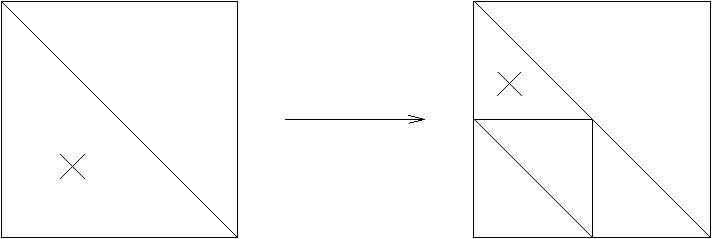
\includegraphics[height=2cm]{pictures/refine_irreg}
\end{center}
But, the obtained mesh is not regular. To avoid such irregular nodes,
also neighboring elements must be split (called green closure):
\begin{center}
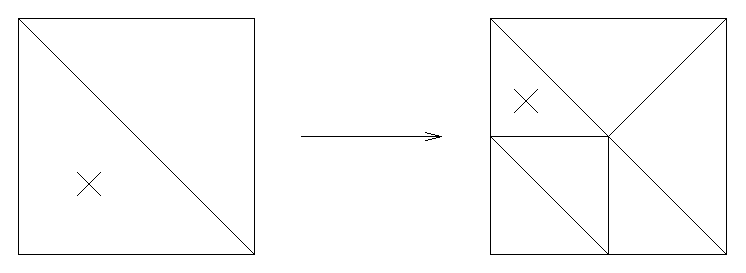
\includegraphics[height=2cm]{pictures/refine_reg}
\end{center}
If one continues to refine that way, the shape of the elements may get worse and worse:
\begin{center}
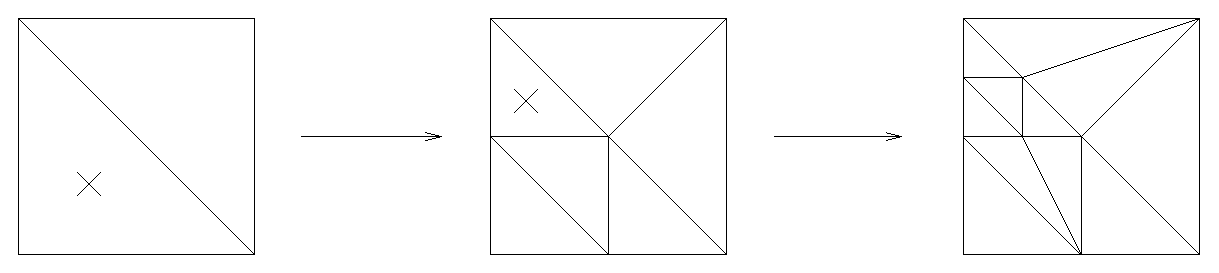
\includegraphics[height=2cm]{pictures/refinebad}
\end{center}
A solution is that elements of the green closure will not be further refined. 
Instead, remove the green closure, and replace it by red refinement. 
\begin{center}
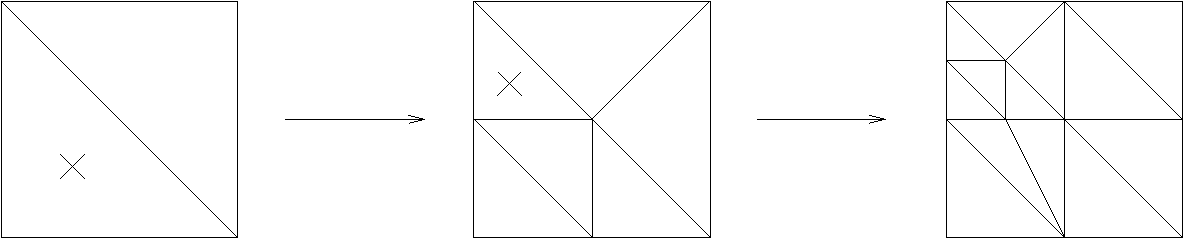
\includegraphics[height=2cm]{pictures/refinegood}
\end{center}


\bigskip
{\bf Marked edge bisection:} \newline
Each triangle has one marked edge. 
The triangle is only refined by cutting from the middle of the
marked edge to the opposite vertex. The marked edges of the new triangles
are the edges of the old triangle.

If there occurs an irregular node, then also the neighbor triangle must be refined.
\begin{center}
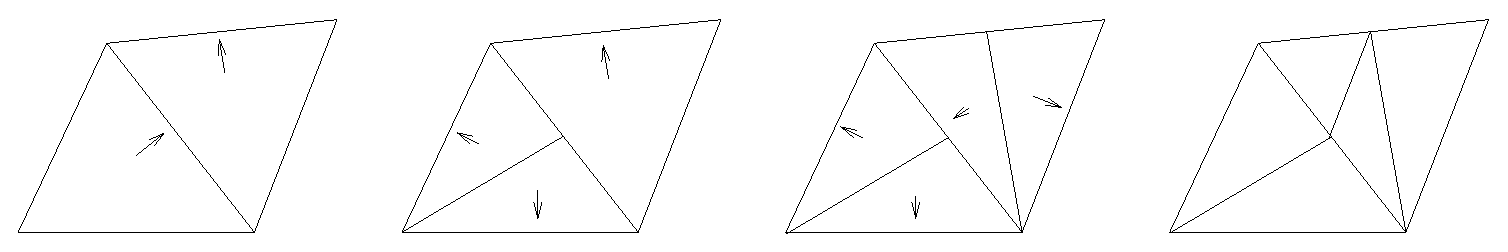
\includegraphics[height=2cm]{pictures/bisect}
\end{center}
To ensure finite termination, one has to avoid cycles in the initial mesh. 
This can be obtained by first sorting the edges (e.g., by length), end then, 
always choose the largest edges as marked edge.

\bigskip

Both of these refinement algorithms are also possible in 3D.

% \documentclass[12pt]{article}
% \usepackage{amsmath,amsthm,amssymb,a4wide}
% \usepackage[german,english]{babel}
% \usepackage{epsfig}
% \usepackage{latexsym}
% \usepackage{amssymb}
% % \usepackage{theorem}
% \usepackage{amsthm}
% % \usepackage{showkeys}

% \newcommand{\setR}{ {\mathbb R} }
% \newcommand{\setN}{ {\mathbb N} }
% \newcommand{\setZ}{ {\mathbb Z} }
% \newcommand{\eps}{\varepsilon}

% \newcommand{\beq}{\begin{equation}}
% \newcommand{\eeq}{\end{equation}}

% \newcommand{\opdiv}{\operatorname{div}}
% \newcommand{\opcurl}{\operatorname{curl}}
% \newcommand{\opdet}{\operatorname{det}}
% \newcommand{\optr}{\operatorname{tr}}
% \newcommand{\optrn}{\operatorname{tr}_n}
% \newcommand{\sfrac}[2]{ { \textstyle \frac{#1}{#2} } }

% \newcommand{\Zh}{\mathrm{Z}_h}
% \newcommand{\Ih}{\mathrm{I}_l}

% \newcommand{\leqc}{\preceq} 
% \newcommand{\geqc}{\succeq} 
% \newcommand{\eqc}{\simeq} 
% \newcommand{\ul}{\underline}

% \newtheorem{theorem}{Theorem}
% \newtheorem{definition}[theorem]{Definition}
% \newtheorem{lemma}[theorem]{Lemma}
% \newtheorem{remark}[theorem]{Remark}
% \newtheorem{example}[theorem]{Example}

% %
% %
% \setlength{\unitlength}{1cm}
% \sloppy 
% %

% \title{Equilibrated Residual Error Estimates}
% \author{Joachim Sch\"oberl}

% \begin{document}
% \maketitle

\section{Equilibrated Residual Error Estimates}

\subsection{General framework}
Equilibrated residual error estimators provide upper bounds for the discretization error in energy norm without any generic constant.
We consider the standard problem: find $u \in V := H_0^1(\Omega)$ such that
$$
\int_\Omega \lambda \nabla u \cdot \nabla v = \int_\Omega f v \qquad \forall \, v \in V
$$
The left hand side defines the bilinear-form $A(\cdot, \cdot)$, the right hand side the linear-form $f(\cdot)$. We define a finite element sub-space $V_h \subset V$ of order $k$, and the finite element solution
$$
\text{find } u_h \in V_h: \quad A(u_h, v_h) = f(v_h) \qquad \forall \, v_h \in V_h.
$$
We assume that $f$ is element-wise polynomial of order $k-1$, and $\lambda$ is element-wise constant and positive.

\qquad

The residual $r(\cdot) \in V^*$ is 
$$
r(v) = f(v) - A(u_h, v) \qquad v \in V
$$
Since 
$$
\| u - u_h \|_A = \sup_{v \in V} \frac{A(u-u_h, v)}{\| v \|_A} = 
 \sup_{v \in V} \frac { r(v) }{\| v \|_A},
$$
we aim in estimating $\|r \|$ in the norm dual to $\| \cdot \|_A$, which is essentially the $H^{-1}$-norm. In general, the direct evaluation of this norm is not feasible.
Using the structure of the problem, we can represent the residual as
$$
r(v) = \sum_{T \in \mathcal{T}} \int_T r_T v + \sum_{E \in \mathcal{E}} \int_E r_E v,
$$
where $r_T$ and $r_E$ are given given as
$$
r_T = f_T + \opdiv \lambda_T \nabla u_{h|T}  \qquad \text{and} \qquad
r_E = \left[  \lambda \frac{\partial u_h} {\partial n}  \right]_E
$$
The element-residual $r_T$ is a polynomial of order $k-1$ on the element $T$, and the edge residual (the normal jump) is a polynomial of order $k-1$ on the edge $E$. 

The {\em residual error estimator} estimates the residual in terms of weighted $L_2$-norms:
$$
\| r \|^2 \eqc \eta^{res}(u_h, f)^2 := \sum_T \frac{ h_T^2}{\lambda_T}  \| r_T \|_{L_2(T)}^2 + \sum_E \frac{ h_E }{\lambda_E} \| r_E \|_{L_2(E)}^2
$$
Here, $\lambda_E$ is some averaging of the coefficients on the two elements containing the edge~$E$. The equivalence holds with constants depending on the shape of elements, the relative jump of the coefficient, and the polynomial order $k$.


The {\em equilibrated residual error estimator} $\eta^{er}$ is defined in terms of the same data $r_T$ and $r_E$. It satisfies
\begin{eqnarray*}
\| u - u_h \|_A & \leq & \eta^{er} \qquad \text{reliable with constant 1} \\
\| u - u_h \|_A & \geq & c \, \eta^{er} \qquad \text{efficient with a generic constant $c$} \\
\end{eqnarray*}
The lower bound depends on the shape of elements and the coefficient $\lambda$, but is robust with respect to the polynomial order $k$.

The main idea is the following: Instead of calculating the $H^{-1}$-norm of $r$, we compute a lifting $\sigma^\Delta$ such that $\opdiv \sigma^\Delta = r$, and calculate the $L_2$-norm of $\sigma^\Delta$. Since $r$ is not a regular function, the equation must be posed in distributional form:
$$
\int_\Omega \sigma^\Delta \cdot \nabla \varphi = - r(\varphi) \qquad \forall \, \varphi \in V
$$
Then, the residual can be estimated without envolving any generic constant:
\begin{eqnarray*}
\| r \|_{A^\ast} & = & \sup_{v \in V} \frac{r(v)}{\| v \|_A} = \sup_v \frac{\int \sigma^\Delta \cdot \nabla v }{\|v \|_A} \\
&= & \sup_v \frac{\int \lambda^{-1/2} \sigma^\Delta \cdot \lambda^{1/2} \nabla v }{\|v \|_A}
\leq \sup_v \frac{\sqrt{\int \lambda^{-1} |\sigma^\Delta|^2}  \sqrt{ \int \lambda |\nabla v|^2 } }{\|v \|_A}
= \| \sigma^\Delta \|_{L_2, 1/\lambda}
\end{eqnarray*}
The norm $\| \sigma^\Delta \| := \int \lambda^{-1} | \sigma^\Delta|^2$ can be evaluated easily. 

Remark: The flux-postprocessing $\sigma := \lambda \nabla u_h + \sigma^\Delta$ provides a flux $\sigma \in H(\opdiv)$ such that $\opdiv \sigma = f$, i.e. the flux is in exact equilibrium with the source $f$. Thus the name.

\subsection{Computation of the lifting $\| \sigma^\Delta \|$}

The residual is a functional of the form
$$
r(v) = \sum_T (r_T, v)_{L_2(T)} + \sum_E (r_E, v)_{L_2(E)},
$$
where $r_T$ and $r_E$ are polynomials of order $k-1$. We search for $\sigma^\Delta$ which is element-wise a vector-valued polynomial of order $k$, and not continuous across edges. Element-wise integration by parts gives
$$
\int_\Omega \sigma \cdot \nabla \varphi = -\sum_T \int_T \opdiv \sigma_{|T} \varphi + \sum_E \int_E [\sigma \cdot n]_E \varphi.
$$
Thus $\opdiv \sigma = r$ in distributional sense reads as
$$
\opdiv \sigma{|T} = r_T \qquad \text{and} \qquad [\sigma \cdot n]_E = -r_E
$$
for all elements $T$ and edges $E$. We could now pose the problem 
$$
\min_{ \sigma \in P^k({\mathcal T})^2 \atop \opdiv \sigma = r} \| \sigma \|_{L_2, 1/\lambda}
$$
We minimize the weighted-$L_2$ norm since we want to find the smallest possible upper bound for the error. This is already a computable approach. 
But, the problem is global, and its solution is of comparable cost as the solution of the original finite element system.  The existence of a $\sigma$ such that $\opdiv \, \sigma = r$ also needs a proof.

We want to localize the construction of the flux. Local problems are associated with vertex-patches $\omega_V = \cup_{T : V \in T} T$. We proceed in two steps:
\begin{enumerate}
\item localization of the residual: $r = \sum_V r^V$
\item local liftings: find $\sigma^V$ such that $\opdiv \sigma^V = r^V$ on the vertex patch
\end{enumerate}
Then, for $\sigma := \sum \sigma^V$ there holds $\opdiv \sigma = r$

The localization is given by multiplication of the $P^1$ vertex basis functions (hat-functions) $\phi_V$:
$$
r^V(v) := r( \phi_V v)
$$
Since $\sum_V \phi_V = 1$, there holds $\sum r^V(\cdot) = r(\cdot)$. The localized residual has the same structure of element and edge terms:
$$
r^V(v) = \sum_{T \subset \omega_V} (r_T^V, v)_{L_2(T)} + \sum_{E \subset \omega_V} (r_E^V, v)_{L_2(E)},
$$
with 
$$
r_T^V = \phi_V r_T \qquad \text{and} \qquad r_E^V = \phi_V r_E
$$
The local residual vanishes on constants on the patch:
$$
r^V(1) = r(\phi_V \, 1) = A(u-u_h, \phi_V) = 0
$$
The last equality follows from the Galerkin-orthogonality. 

We give an explicit construction of the lifting $\sigma^V$ in terms of the Brezzi-Douglas-Marini (BDM) element. The $k^{th}$ order BDM element on a triangle is given by $V_T = [P^k]^2$ and the degrees of freedom:
\begin{enumerate}
\item[(i)] $\int_E \sigma\cdot n \, q_i$  with $q_i$ a basis for $ P^k(E)$
\item[(ii)] $\int_T \opdiv \sigma \, q_i$  with $q_i$ a basis for $ P^{k-1}(T) \cap L_2^0(T)$
\item[(iii)] $\int_T \sigma \cdot \opcurl q_i$  with $q_i$ a basis for $ P_0^{k+1}(T)$
\end{enumerate}
Exercise: Show that these dofs are unisolvent. Count dimensions, and prove that $[ \forall i: \psi_i(\sigma) =0 ] \Rightarrow \sigma = 0$.


Now, we give an explicit construction of equilibrated fluxes on a vertex patch. Label elements $T_1, T_2, \ldots T_n$ in a counter-clock-wise order. Edge $E_i$ is the  common edge between triangle $T_{i-1}$ and $T_i$ (with identifying $T_0 = T_n$). We define $\sigma$ by specifying the dofs of the BDM element:
\begin{enumerate}
\item
Start on $T_1$. We set $\sigma_n = -r^V_{E_1}$ on edge $E_1$. On the edge on the patch-boundary we set $\sigma_n = 0$, and on $E_2$ we set $\sigma_n = const$ such that $\int_{\partial T_1} \sigma_n = \int_{T_1} r^V_T$. We use the dofs of type (ii) to specify 
$\int_T \opdiv \sigma \, q = \int_T r_T^V q \; \forall q \in P^{k-1} \cap L_2^0(T)$. Together with get $\opdiv \sigma = r_T$. Dofs of type (iii) are not needed, and set 0. There holds
$$
\int_{E_2} \sigma_n = \int_{T_1} r^V_T - \int_{E_1} \sigma_n = \int_{T_1} r^V_{T_1} + \int_{E_1} r^V_{E_1}
$$
\item Continue with element $T_2$. On edge $E_2$ common with $T_1$ set $\sigma_n$ such that $[\sigma \cdot n]_{E_2} = r_{E_2}$. Otherwise, proceed as on $T_1$. Thus
$$
\int_{E_3} \sigma_n = \int_{T_1} r^V_{T_1} + \int_{E_1} r^V_{E_1} +\int_{T_2} r^V_{T_2} + \int_{E_2} r^V_{E_2} 
$$
\item Continue to element $T_n$. Observe that on $T_n$:
$$
\int_{E_1} \sigma_n = \sum_{i=1}^n \int_{T_i} r^V_{T_i} + \sum_{i=1}^n \int_{E_i} r^V_{E_i} = 0,
$$
which follows from $r^V(1) = 0$. Thus, also $[\sigma \cdot n]_{E_1} = r_{E_1}^V$ is satisfied.
\end{enumerate}

This explicit construction proves the existence of an equilibrated flux. Instead of this explicit construction, one may solve a local constrained optimization problem
$$
\min_{\sigma^V : \opdiv \sigma^V = r^V} \| \sigma \|_{L_2, \lambda^{-1}}
$$
This applies also for 3D. Furthoer notes
\begin{itemize}
\item mixed boundary conditions are possible
\item the efficiency for the h-FEM is shown by scaling arguments, and equivalence to the residual error estimator
\item efficiency is also proven to be robust with respect to polynomial order $k$, examples show overestimation less than 1.5
\end{itemize}


\bigskip \noindent 
{\bf Literature:}
\begin{enumerate}
\item 
D. Braess and J. Sch\"oberl.
\newblock  Equilibrated Residual Error Estimator for Maxwell's
Equations.
\newblock {\em Mathematics of Computation}, Vol 77(262), 651-672, 2008
\item 
D. Braess, V. Pillwein and J. Sch\"oberl: 
\newblock Equilibrated Residual Error Estimates are p-Robust. Computer
\newblock {\em Methods in Applied Mechanics and Engineering.} Vol 198,
1189-1197, 2009
\end{enumerate}



% \end{document}

\section{Non-conforming Finite Element Methods}
\label{sec_nonconforming}
In a conforming finite element method, one chooses a sub-space $V_h \subset V$, and defines the finite element approximation as
$$
\mbox{Find } u_h \in V_h: \qquad A(u_h, v_h) = f(v_h) \qquad \forall \, v_h \in V_{h}
$$
For reasons of simpler implementation, or even of higher accuracy, the 
conforming framework is often violated. Examples are:
\begin{itemize}
\item
The finite element space $V_h$ is not a sub-space of $V = H^m$. 
Examples are the non-conforming $P^1$ triangle, and the Morley element for
approximation of $H^2$.
\item
The Dirichlet boundary conditions are interpolated in the boundary vertices.
\item
The curved domain is approximated by straight sided elements
\item
The bilinear-form and the linear-form are approximated  by 
inexact numerical integration
\end{itemize}

\noindent
The lemmas by Strang are the extension of Cea's lemma to the 
non-conforming setting.


\subsubsection{The First Lemma of Strang}
In the first step, let $V_h \subset V$, but the bilinear-form and the linear-form are replaced by mesh-dependent forms 
$$
A_h(.,.): V_h \times V_h \rightarrow \setR
$$ 
and 
$$
f_h(.) : V_h \rightarrow \setR.
$$
We do not assume that $A_h$ and $f_h$ are defined on $V$. 
We assume that the bilinear-forms $A_h$ are uniformly coercive, i.e.,
there exists an $\alpha_1$ independent of the mesh-size such that
$$
A_h (v_h, v_h) \geq \alpha_1 \, \| v_h \|_V^2 \qquad \forall \, v_h \in V_h
$$
The finite element problem is defined as 
$$
\mbox{Find } u_h \in V_h: \qquad A_h (u_h, v_h) = f_h (v_h) \qquad \forall \, v_h \in V_h
$$

\begin{lemma}[First Lemma of Strang] Assume that
\begin{itemize}
\item $A(.,.)$ is continuous on $V$
\item $A_h(.,.)$ is uniformly coercive 
\end{itemize}
Then there holds
\begin{eqnarray*}
\| u - u_h \| & \leqc & \inf_{v_h \in V_h} \left\{
        \| u - v_h \| + \sup_{w_h \in V_h} \frac{|A(v_h, w_h) - A_h (v_h, w_h)|}{\| w_h \|} \right\} \\
        & & 
        + \sup_{w_h \in V_h} \frac{f(w_h) - f_h (w_h)}{\| w_h \|}
\end{eqnarray*}
\end{lemma}     
{\em Proof:} 
Choose an arbitrary $v_h \in V_h$, and set $w_h := u_h - v_h$.
We use the uniform coercivity, and the definitions of $u$ and $u_h$:
\begin{eqnarray*}
\alpha_1 \| u_h - v_h \|_V^2 & \leq & A_h (u_h - v_h, u_h - v_h) = A_h (u_h - v_h, w_h) \\
        & = & A(u-v_h, w_h) + [ A(v_h, w_h) - A_h(v_h, w_h) ] + [ A_h (u_h, w_h) - A(u, w_h)] \\
        & = & A(u-v_h, w_h) + [ A(v_h, w_h) - A_h(v_h, w_h) ] + [ f_h(w_h) - f(w_h)]
\end{eqnarray*}
Divide by $\| u_h - v_h \| = \| w_h \|$, and use the continuity of $A(.,.)$:
\begin{equation}
\label{equ_strang1a}
\| u_h - v_h \| \leqc \| u - v_h \| + \frac{|A(v_h, w_h) - A_h(v_h, w_h)|}{\| w_h  \|} + \frac{ | f(w_h) - f_h(w_h) | } { \| w_h \| }
\end{equation}

Using the triangle inequality, the error $\| u - u_h \|$ is bounded by
$$
\| u - u_h \| \leq \inf_{v_h \in V_h} \| u - v_h \| + \| v_h - u_h \|
$$
The combination with (\ref{equ_strang1a}) proves the result. 
\hfill $\Box$

\bigskip

{\bf Example:} Lumping of the $L_2$ bilinear-form: \newline
Define the $H^1$ - bilinear-form
$$
A(u,v) = \int_\Omega \nabla u \cdot \nabla v + \int_\Omega u v \, dx,
$$
and perform Galerkin discretization with $P^1$ triangles.
The second term leads to a non-diagonal matrix. 
The vertex integration rule
$$
\int_T v \, dx \approx \frac{|T|}{3} \sum_{\alpha = 1}^3 v(x_{T,\alpha})
$$
is exact for $v \in P^1$. We apply this integration rule for the term
$\int u v \, dx$:
$$
A_h(u,v) = \int \nabla u \cdot \nabla v + 
\sum_{T \in {\cal T}} \frac{|T|}{3} \sum_{\alpha = 1}^3 u(x_{T,\alpha}) v(x_{T,\alpha})
$$
The bilinear form is now defined only for $u, v \in V_h$.
The integration is not exact, since $u v \in P^2$ on each triangle.

Inserting the nodal basis $\varphi_i$, we obtain a diagonal matrix for
the second term:
$$
\varphi_i (x_{T,\alpha}) \varphi_j (x_{T,\alpha}) = 
        \left\{ \begin{array}{cl}
                1 & \mbox{for } x_i = x_j = x_{T,\alpha} \\
                0 & \mbox{else}
        \end{array}
        \right.
$$

To apply the first lemma of Strang, we have to verify the uniform coercivity
\begin{equation}
\label{equ_uniformell}
\sum_T \frac{|T|}{3} \sum_{\alpha = 1}^3 |v_h(x_{T,\alpha})|^2 \geq 
\alpha_1 \sum_T \int_T | v_h |^2 \, dx \qquad \forall \, v_h \in V_h,
\end{equation}
which is done by transformation to the reference element.
The consistency error can be estimated by
\begin{equation}
\label{equ_consist}
| \int_T u_h v_h \, dx - \frac{|T|}{3} \sum_{\alpha=1}^3 u_h(x_\alpha) v_h(x_\alpha) |
 \leqc h_T^2 \, \| \nabla u_h \|_{L_2(T)} \, \| \nabla v_h \|_{L_2(T)}
\end{equation}
Summation over the elements give
$$
A(u_h, v_h) - A_h (u_h, v_h) \leqc h^2 \| u_h \|_{H^1(\Omega)} \, \| v_h \|_{H^1(\Omega)}
$$
The first lemma of Strang proves that this modification of the bilinear-form
preserves the order of the discretization error:
\begin{eqnarray*}
\| u - u_h \|_{H^1} & \leqc & 
 \inf_{v_h \in V_h} \left\{
        \| u - v_h \|_{H^1} + \sup_{w_h \in V_h} \frac{|A(v_h, w_h) - A_h (v_h, w_h)|}{\| w_h \|_{H^1}} \right\} \\
 & \leqc & 
        \| u - I_h u \|_{H^1} + \sup_{w_h \in V_h} \frac{|A(I_h u, w_h) - A_h (I_h u, w_h)|}{\| w_h \|_{H^1}} \\
 & \leqc &  h \, \| u \|_{H^2} + \sup_{w_h \in V_h} \frac{h^2 \, \| I_h u \|_{H^1} \| w_h \|_{H^1}}{\| w_h \|_{H^1}} \\
 &  \leqc & h \, \| u \|_{H^2}
\end{eqnarray*}

A diagonal $L_2$ matrix has some advantages:
\begin{itemize}
\item It avoids oscillations in boundary layers (exercises!)
\item In explicit time integration methods for parabolic or hyperbolic
problems, one has to solve linear equations with the $L_2$-matrix. This
becomes cheap for diagonal matrices.
\end{itemize}

\subsubsection{The Second Lemma of Strang}

In the following, we will also skip the requirement $V_h \subset V$. 
Thus, the norm $\|.\|_V$ cannot be used on $V_h$, and it will be replaced by
mesh-dependent norms $\|.\|_h$. These norms must be defined for $V + V_h$.
As well, the mesh-dependent forms $A_h(.,.)$ and $f_h(.)$ are defined 
on $V + V_h$. We assume 
\begin{itemize}
\item uniform coercivity:
$$
A_h (v_h, v_h) \geq \alpha_1 \| v_h \|_h^2 \qquad \forall \, v_h \in V_h
$$
\item continuity:
$$
A_h (u, v_h) \leq \alpha_2 \| u \|_h \| v_h \|_h \qquad \forall \, u \in V + V_h, \; \forall \, v_h \in V_h
$$
\end{itemize}

The error can now be measured only in the discrete norm $\| u - u_h \|_{V_h}$.
\begin{lemma}
Under the above assumptions there holds
\begin{equation}
\label{equ_strang2}
\| u - u_h \|_h \leqc \inf_{v_h \in V_h} \| u - v_h \|_h +
         \sup_{w_h \in V_h} \frac{| A_h(u,w_h) - f_h(w_h) |}{\| w_h \|_h}
\end{equation}
\end{lemma}
{\em Remark}: The first term in (\ref{equ_strang2}) is the approximation
error, the second one is called consistency error. \\
{\em Proof:} Let $v_h \in V_h$. Again, set $w_h = u_h - v_h$, and
use the $V_h$-coercivity:
\begin{eqnarray*}
\alpha_1 \, \| u_h - v_h \|_h^2 & \leq & A_h (u_h - v_h, u_h - v_h) = A_h (u_h - v_h, w_h) \\
        & = & A_h (u-v_h, w_h) + [f_h(w_h) - A_h(u,w_h)]
\end{eqnarray*}
Again, divide by $\| u_h - v_h\|$, and use continuity of $A_h(.,.)$:
$$
\| u_h - v_h \|_h \leqc \| u - v_h \|_h + \frac{A_h(u,w_h) - f_h(w_h)}{\| w_h \|_h}
$$
The rest follows from the triangle inequality. \hfill $\Box$


\subsubsection{The non-conforming $P^1$ triangle}

The non-conforming $P^1$ triangle is also called the Crouzeix-Raviart element.

The finite element space generated by the non-conforming $P^1$ element
is
$$
V_h^{nc} := \{ v \in L_2 : v_{|T} \in P^1(T), \mbox{and }v \mbox{ is continuous in edge mid-points} \}
$$

The functions in $V_h^{nc}$ are not continuous across edges, and thus, 
$V_h^{nc}$ is not a sub-space of $H^1$. We have to extend the bilinear-form and
the norm in the following way:
$$
A_h (u,v) = \sum_{T \in {\cal T}} \int_T \nabla u \nabla v \, dx
        \qquad \forall \, u, v \in V + V_h^{nc}
$$
and
$$
\| v \|_h^2 := \sum_{T \in {\cal T}}  \| \nabla v \|_{L_2(T)}^2 \qquad \forall \, v \in V + V_h^{nc}
$$


We consider the Dirichlet-problem with $u = 0$ on $\Gamma_D$. 


We will apply the second lemma of Strang.

The continuous $P^1$ finite element space $V_h^c$ is a sub-space of 
$V_h^{nc}$. Let $I_h : H^2 \rightarrow V_h^c$ be the nodal interpolation
operator.

To bound the approximation term in (\ref{equ_strang2}), we use the
inclusion $V_h^c \subset V_h^{nc}$:
$$
\inf_{v_h \in V_h^{nc}} \| u - v_h \|_h \leq \| u - I_h u \|_{H^1} \leqc h \, \| u \|_{H^2}
$$


We have to bound the consistency term
\begin{eqnarray*}
r(w_h) & = & A_h(u,w_h) - f(w_h) \\
        & = & \sum_T \int_T \nabla u \nabla w_h - \sum_T \int_T f w_h \, dx \\
        & = & \sum_T \int_{\partial T} \frac{\partial u}{\partial n} w_h \, ds 
                - \sum_T \int_T (\Delta u + f) \, w_h \, ds \\
        & = & \sum_T \int_{\partial T} \frac{\partial u}{\partial n} w_h \, ds 
\end{eqnarray*}


Let $E$ be an edge of the triangle $T$. Define the mean value $\overline{w_h}^E$. 
If $E$ is an inner edge, then the mean value on the corresponding edge of
the neighbor element is the same. The normal derivative $\frac{\partial u}{\partial n}$ on the neighbor element is (up to the sign) the same.
If $E$ is an edge on the Dirichlet boundary, then the mean value is 0.
This allows to subtract edge mean values:

$$
r(w_h) = \sum_T \sum_{E \subset T} \int_E \frac{\partial u}{\partial n} (w_h - \overline{w_h}^E) \, ds
$$
Since $\int_E w_h - \overline{w_h}^E \, ds = 0$, we may insert the 
constant function $\frac{\partial I_h u}{\partial n}$ on each edge:
$$
r(w_h) = \sum_T \sum_{E \subset T} \int_E 
        \left(\frac{\partial u}{\partial n} - \frac{\partial I_h u}{\partial n} \right) (w_h - \overline{w_h}^E) \, ds
$$
Apply Cauchy-Schwarz on $L_2(E)$:
$$
r(w_h) = \sum_T \sum_{E \subset T} \| \nabla (u - I_h u) \|_{L_2(E)} \| w_h - \overline{w_h}^E \|_{L_2(E)}
$$

To estimate these terms, we transform to the reference element $\widehat T$, 
where we apply the Bramble Hilbert lemma. Let $T = F_T(\widehat T)$, and set
$$
\widehat u = u \circ F_T \qquad \widehat w_h = w_h \circ F_T
$$
There hold the scaling estimates
\begin{eqnarray*}
| w_h |_{H^1(T)} & \eqc & | \widehat w_h |_{H^1(\widehat T)} \\
\| w_h - \overline {w_h}^E \|_{L_2(E)} & \eqc & h_E^{1/2} \| \widehat w_h - \overline{\widehat w_h}^{\widehat E} \|_{L_2(\widehat E)} \\
| u |_{H^2(T)} & \eqc & h_T^{-1} |  \widehat u |_{H^2(\widehat T)} \\
\| \nabla (u - I_h u) \|_{L_2(E)} & \eqc & h_E^{-1/2} \| \nabla (\widehat u - \widehat I_h \widehat u) \|_{L_2(E)}
\end{eqnarray*}
On the reference element, we apply the Bramble Hilbert lemma, once for $w_h$, 
and once for $u$. The linear operator 
$$
L : H^1(\widehat T) \rightarrow L_2(\widehat E) :
 \widehat w_h \rightarrow  \widehat w_h - \overline {\widehat w_h}^{\widehat E}
$$
is bounded on $H^1(\widehat T)$ (trace theorem), and $L w = 0$ for $w \in P_0$,
thus
$$
\| \widehat w_h - \overline{\widehat w_h}^{\widehat E} \|_{L_2(\widehat E)}
\leqc | \widehat w_h |_{H^1(\widehat T)}
$$
Similar for the term in $u$: There is $\| \nabla (u - I_h u) \|_{L_2(E)} \leqc \| u \|_{H^2(T)}$, and $u - I_h u$ vanishes for $u \in P^1$. 

Rescaling to the element $T$ leads to
\begin{eqnarray*}
\| w_h - \overline{w_h}^E \|_{L_2(E)} & \leqc & h^{1/2} \, | w_h |_{H^1(T)} \\
\| \nabla (u - I_h u) \|_{L_2(E)} & \leqc & h^{1/2} \, | u |_{H^2(T)}
\end{eqnarray*}
This bounds the consistency term
$$
r(w_h) \leqc \sum_T h \, | u |_{H^2(T)} | w_h |_{H^1(T)} \leqc h \, \| u \|_{H^2(\Omega)} \, \| w_h \|_h.
$$
The second lemma of Strang gives the error estimate
$$
\| u - u_h \| \leqc h \, \| u \|_{H^2}
$$ 

There are several applications where the non-conforming $P^1$ triangle
is of advantage:
\begin{itemize}
\item
The $L_2$ matrix is diagonal (exercises)
\item
It can be used for the approximation of problems in fluid dynamics
described by the Navier Stokes equations (see later).
\item
The finite element matrix has exactly 5 non-zero entries in each row
associated with inner edges. That allows simplifications in the matrix
generation code.
\end{itemize}

% \documentclass[12pt]{article}
% \usepackage{amsmath,amsthm,amssymb,a4wide}
% \usepackage[german,english]{babel}
% \usepackage{epsfig}
% \usepackage{latexsym}
% \usepackage{amssymb}
% % \usepackage{theorem}
% \usepackage{amsthm}
% % \usepackage{showkeys}

% \newcommand{\setR}{ {\mathbb R} }
% \newcommand{\setN}{ {\mathbb N} }
% \newcommand{\setZ}{ {\mathbb Z} }
% \newcommand{\eps}{\varepsilon}

% \newcommand{\beq}{\begin{equation}}
% \newcommand{\eeq}{\end{equation}}

% \newcommand{\opdiv}{\operatorname{div}}
% \newcommand{\opcurl}{\operatorname{curl}}
% \newcommand{\opdet}{\operatorname{det}}
% \newcommand{\optr}{\operatorname{tr}}
% \newcommand{\optrn}{\operatorname{tr}_n}
% \newcommand{\sfrac}[2]{ { \textstyle \frac{#1}{#2} } }

% \newcommand{\Zh}{\mathrm{Z}_h}
% \newcommand{\Ih}{\mathrm{I}_l}

% \newcommand{\leqc}{\preceq} 
% \newcommand{\geqc}{\succeq} 
% \newcommand{\eqc}{\simeq} 
% \newcommand{\ul}{\underline}

% \newtheorem{theorem}{Theorem}
% \newtheorem{definition}[theorem]{Definition}
% \newtheorem{lemma}[theorem]{Lemma}
% \newtheorem{remark}[theorem]{Remark}
% \newtheorem{example}[theorem]{Example}

% %
% %
% \setlength{\unitlength}{1cm}
% \sloppy 
% %

% \title{hp - Finite Elements}
% \author{Joachim Sch\"oberl}

% \begin{document}
% % \selectlanguage{german}

% \maketitle

\section{hp - Finite Elements}

Let $V_{hp}$ be a $p$-th order finite element sub-space of $H^1$.
By scaling and Bramble-Hilbert technique one obtains the best-approxiamtion error estimate
$$
\inf_{v_{hp} \in V_{hp}} \| u - v_{hp} \|_{H^1}  \leq c h^{m-1} \| u \|_{H^m}
$$
for $m \leq p+1$. The constant $c$ depends on the order $p$. If $m$ is fixed, we do obtain reduction of the approximation error as we increase $p$. Next we develop methods to obtain so called $p$-version error estimates 
$$
\inf_{v_{hp} \in V_{hp}} \| u - v_{hp} \|_{H^1}  \leq c \left( \sfrac{h}{p} \right) ^{m-1} \| u \|_{H^m},
$$
where $c$ is independent of $h$ and $p$. This estimate proves also convergence of the $p$-version finite element method: One may fix the mesh, and increase the order $p$. 

A detailed analyis of local $H^m$ norms allows an optimal balance of
mesh-size $h$ and polynomial order $p$. This $hp$-version leads to
exponential convergence
$$
\inf_{v_{hp} \in V_{hp}} \| u - v_{hp} \|_{H^1}  \leq c e^{ -N^\alpha },
$$
where $N$ is the number of unknowns. 
 
We will prove the $p$-version estimate, but not the $hp$-result.

\subsection{Legendre Polynomials}
Orthogonal polynomials are important to construct stable basis 
functions for the $p$-FEM, as well as for error estimates.

Let $\Pi_n$ denote the space of polynomials up to order $n$. We write $\pi_n$ for 
a generic polynomial in $\Pi_n$, with a different value any time it appears.

Definition of Legendre polynomials via Rodrigues' formula:
$$
P_n(x) := \frac{1}{2^n n!} \frac{d^n}{dx^n} (x^2-1)^n.
$$
It is a polynomial of degree $n$. The first few Legendre polynomials are
\begin{eqnarray*}
P_0(x) & = & 1 \\
P_1(x) & = & x \\
P_2(x) & = & \sfrac{3}{2} x^2 - \sfrac{1}{2}
\end{eqnarray*}
$P_n$ is even if $n$ is even, and $P_n$ is odd if $n$ is odd.
Since $(x^2-1)^n = x^{2n} - n x^{2n-2} + \pi_{2n-4}$ (with proper
modification for small $n$) we have
\begin{equation}
\label{equ_leadingcoef}
P_n(x) = \frac{1}{2^n n!} \frac{ (2n)! }{ n! } x^n - \frac{n}{2^n n!} \frac{ (2n-2)!} {(n-2)!} x^{n-2} + \pi_{n-4}
\end{equation}
\begin{lemma} \label{lemma_ortho} There holds
\begin{equation} \label{equ_ortho}
\int_{-1}^1 P_n(x) P_m(x) \, dx = \frac{2}{2n+1} \delta_{n,m}.
\end{equation}
\end{lemma}
\begin{proof} W.l.o.g. let $n \leq m$. Multiple integration by parts gives
\begin{eqnarray*}
\lefteqn{ 2^{n+m} n! m! \int_{-1}^1 P_n(x) P_m(x) \, dx = 
\int_{-1}^1 \frac{d^n}{dx^n} (x^2-1)^n \frac{d^m}{dx^m} (x^2-1)^n  \, dx}
\\
& = & \int_{-1}^1 \frac{d^{n+1}}{dx^{n+1}} (x^2-1)^n \frac{d^{m-1}}{dx^{m-1}} (x^2-1)^m 
+ 
\left[ \frac{d^n}{dx^{n}} (x^2-1)^n \underbrace{ \frac{d^{m-1}}{dx^{m-1}} (x^2-1)^m}_{= 0 \text{ for } x \in \{ -1, 1\}} \right]_{-1}^1 \\
& = & \cdots \\
& = & \int_{-1}^1 \frac{d^{n+m}}{dx^{n+m}} (x^2-1)^n (x^2-1)^m \, dx
\end{eqnarray*} 
For $n < m$, the first factor of the integrand vanishes, and we have orthogonality. For $n = m$ this equals
\begin{eqnarray*}
2^{2n} (n!)^2 \| P_n \|_{L_2}^2 &= &\int_{-1}^1 (2n)! (x^2-1)^n \, dx = (2n)! \int_{-1}^1 (x-1)^n (x+1)^n \\
& = & -(2n)! \int_{-1}^1 \frac{n}{n+1} (x-1)^{n+1} (x+1)^{n-1} \\
& = & (2n)! \int_{-1}^1 \frac{ n (n-1) }{ (n+1) (n+2) } (x-1)^{n+2}(x+1)^{n-2} = ...  \\
& = & (2n)! \frac{n!} {2n (2n-1) \cdots (n+1)} \int_{-1}^1 (x-1)^{2 n} \, dx = (n!)^2 \frac{1}{2n+1} \, 2^{2n+1},
\end{eqnarray*}
which proves the scaling.
\end{proof}

Next we prove the 3-term recurrency, which can be used for efficient evaluation.
\begin{lemma} \label{lemma_threeterm} There holds
\begin{equation} \label{equ_threeterm}
(n+1) P_{n+1} (x) = (2n+1) x P_n(x) - n P_{n-1}(x).
\end{equation}
\end{lemma}
\begin{proof} Set $r(x) = (n+1) P_{n+1} (x) - (2n+1) x P_n(x) + n P_{n-1}(x)$.
Using (\ref{equ_leadingcoef}), we see that the leading coefficients cancel, 
and thus $r \in \Pi_{n-2}$. From Lemma~\ref{lemma_ortho} we get for 
any $q \in \Pi_{n-2}$
$$
\int_{-1}^1 r(x) q(x) \, dx = (n+1) \int_{-1}^1 P_{n+1} \, q - (2n+1) \int_{-1}^1 P_n \underbrace{x q}_{\in \Pi_{n-1}} + n \int_{-1}^1 P_{n-1} \, q = 0,
$$
and thus $r = 0$. 
\end{proof} 

\begin{lemma} \label{lemma_sturmliouville} Legendre polynomials satisfy the Sturm-Liouville differential equation
$$
\frac{d}{dx} \big[ (x^2-1) \frac{d}{dx} P_n(x) \big] = n (n+1) P_n(x)
$$
\end{lemma} 
\begin{proof} Both sides are in $\Pi_n$. We compare leading coefficients, for this set $P_n = a_n x^n + \pi_{n-2}$ (with $a_n =  \frac{1}{2^n n!} \frac{ (2n)! }{ n! }$).
\begin{eqnarray*}
lhs & = & \frac{d}{dx} \left[ (x^2-1) \frac{d}{dx} \left( a_n x^n + \pi_{n-2} \right) \right] \\
& = & \frac{d}{dx} \left[ (x^2-1) (a_n n x^{n-1} + \pi_{n-3}) \right] \\
& = & \frac{d}{dx} \left[ a_n n x^{n+1} + \pi_{n-1} \right] \\
& = & n (n+1) a_n x^n + \pi_{n-2}, 
\end{eqnarray*}
and we get the same leading coefficient for rhs. Furthermore, for $q \in \Pi_{n-1}$ there holds
\begin{eqnarray*}
\int_{-1}^1 lhs \, q & = &-\int_{-1}^1 (x^2-1) P_n^\prime q^\prime \, dx + \underbrace{ \left[ (x^2-1) P_n^\prime q \right]_{-1}^1 }_{= 0} \\
& = & \int_{-1}^1 P_n \underbrace{ \left( (x^2-1) q^\prime\right)^\prime}_{\in \Pi_{n-1}} \, dx - \left[ P_n (x^2-1) q^\prime \right]_{-1}^1 = 0,
\end{eqnarray*}
and the same for the rhs. Thus the identity is proven.
\end{proof}

Lemma~\ref{lemma_sturmliouville} implies that the Legendre polynomials are also orthogonal w.r.t. $(u^\prime, v^\prime)_{L_2, 1-x^2}$, i.e.
$$
\int_{-1}^1 (1-x^2) P_n^\prime P_m^\prime = n(n+1) \| P_n \|_{L_2}^2 \delta_{n,m}
$$


\subsection{Error estimate of the $L_2$ projection}
Since polynomials are dense in $L_2(-1,1)$, we get
$$
u = \sum_{n=0}^\infty a_n P_n
$$
with the generalized Fourier coefficients
$$
a_n = \frac{ (u, P_n)_{L_2} } { \| P_n \|^2_{L_2} },
$$
and
$$
\| u \|_{L_2}^2 = \sum_{n=0}^\infty a_n^2 \| P_n \|^2.
$$
Let $P_{L_2}^{\Pi_p}$ denote the $L_2$-projection onto $\Pi_p$. There holds
$$
P_{L_2}^{\Pi_p} u = \sum_{n=0}^p a_n P_n
$$
The projection error is
$$
\| u - P_{L_2}^{\Pi_p} u \|_{L_2}^2 = \sum_{n=p+1}^\infty a_n^2 \| P_n \|^2
$$
\begin{lemma} \label{lemma_l2est}  The $L_2$-projection error satisfies
\begin{equation}
\| u - P_{L_2}^{\Pi_p} u \|_{L_2(-1,1)} \leq \frac{1}{\sqrt{(p+1)(p+2)}} \, | u |_{H^1(-1,1)}
\end{equation}
\end{lemma}
\begin{proof} Since $P_n$ are orthogonal also w.r.t. $(u^\prime, v^\prime)_{L_2, 1-x^2}$,
there holds
$$
\| u^\prime \|_{L_2, 1-x^2}^2 = \sum_{n \in \setN} a_n^2 \, \| P_n^\prime \|_{1-x^2}^2,
$$
provided that $u$ is in $H^1$.
The projection error satisfies
\begin{eqnarray*}
\| u - P_{L_2}^{\Pi_p} u \|^2_{L_2} & = & \sum_{n > p} a_n^2 \| P_n \|^2_{L_2} 
 = \sum_{n > p} a_n^2 \frac{1}{n (n+1)} \| P_n^\prime \|^2_{1-x^2} \\
& \leq & \frac{1}{(p+1)(p+2)} \sum_{n > p} a_n^2 \|P_n^\prime \|^2_{1-x^2} 
\leq  \frac{1}{(p+1)(p+2)} \sum_{n \in \setN} a_n^2 \|P_n^\prime \|^2_{1-x^2} \\
& = & \frac{1}{(p+1)(p+2)} \| u^\prime \|_{1-x^2}^2 \\
\end{eqnarray*}
Finally, the result follows from 
$$
\int_{-1}^1 (1-x^2) (u^\prime)^2 \, dx \leq \int_{-1}^1 (u^\prime)^2 \, dx.
$$
\end{proof}
\newpage
Similar as in Lemma~\ref{lemma_sturmliouville} on shows also
$$
\frac{d^m}{dx^m} \big[ (x^2-1)^m \frac{d^m}{dx^m} P_n(x) \big] = (n+m)(n+m-1) \ldots (n-m+1) P_n(x)
$$
for $m \leq n$, and, as in Lemma~\ref{lemma_l2est}
$$
\| u - P_{L_2}^{\Pi_p} u \|_{L_2} \leq \sqrt{ \frac{ (p-m+1)! }{ (p+m+1)! } } | u |_{H^m}.
$$


\subsection{Orthogonal polynomials on triangles}
%
Orthogonal polynomials on tensor product elements are simply
constructed by tensorization. Orthogonal polynomials on simplicial
elements are more advanced. They are based on Jacobi polynomials:

For $\alpha, \beta > -1$, Jacobi polynomials are defined by 
$$
P_n^{(\alpha, \beta)}(x) := \frac{(-1)^n}{2^n n!} \frac{1}{w(x)} \frac{d^n}{dx^n} \big( w(x) (1-x^2)^n \big)
$$
with the weight function 
$$
w(x) = (1-x)^\alpha (1+x)^\beta.
$$
Jacobi polynomials are orthogonal w.r.t. the weighted inner product
$$
\int_{-1}^1 w(x) P_n^{(\alpha,\beta)}(x) P_m^{(\alpha, \beta)}(x) dx = \delta_{n,m} \frac{2^{\alpha+\beta+1}}{2n+\alpha+\beta+1} \frac{ \Gamma(n+\alpha+1) \, \Gamma (n+\beta+1) } { n! \Gamma (n+\alpha+\beta+1)}.
$$
Note that $P^{(0,0)}_n = P_n$.

Define the unit-triangle $T$ with vertices $(-1,0)$,  $(1,0)$ and $(0,1)$. 
\begin{lemma} [Dubiner basis] The functions
$$
\varphi_{i,j} (x,y) := P_i \big( \sfrac{x}{1-y} \big) (1-y)^i P_j^{(2i+1,0)} (2y-1)
\qquad i+j \leq p
$$ 
form an $L_2(T)$-orthogonal basis for $\Pi_p(T)$.
\end{lemma}
\begin{proof}
Note that $\varphi_{i,j} \in \Pi_{i+j}$. Substitution $\xi = \frac{x}{1-y}$ leads to
\begin{eqnarray*}
\lefteqn{ \int_T \varphi_{ij}(x,y) \varphi_{kl} (x,y) \, d(x,y) = } \\
& = & \int_0^1 \int_{-1+y}^{1-y} 
 P_i \big( \sfrac{x}{1-y} \big) (1-y)^i P_j^{(2i+1,0)} (2y-1)
 P_k \big( \sfrac{x}{1-y} \big) (1-y)^k P_l^{(2k+1,0)} (2y-1) \, dx dy \\
& = & \int_0^1 \int_{-1}^1 P_i(\xi) P_k(\xi) (1-y)^{i+k+1} P_j^{(2i+1,0)} (2y-1) P_l^{(2k+1,0)}(2y-1) \, d\xi dy \\
& = & \delta_{i,k} \| P_i \|_{L_2}^2 \int_0^1 (1-y)^{2i+1} P_j^{(2i+1,0)}(2y-1) P_l^{(2i+1,0)}(2y-1) \, dy \\
& = & C_{ij} \delta_{i,k} \delta_{j,l} 
\end{eqnarray*}
\end{proof}



\subsection{Projection based interpolation}

By means of the orthogonal polynomials one shows approximation error estimates
of the form
$$
\inf_{q \in \Pi_p(T)} \| u - q \|_{H^k(T)} \leq c p^{k-m} | u |_{H^m(T)} \qquad m \geq k,
$$
with $c \neq c(p)$, easily in 1D and tensor product elements, and also on $n$-dimensional simplices [Braess+Schwab: Approximation on simplices with respect to weighted Sobolev norms, J. Approximation Theory 103, 329-337 (2000)].
 
But, an interpolation operator to an $H^1$-conforming finite element space has to satisfy continuity constraints across element boundaries. We show that we get the same rate of convergence under these constraints.

\subsubsection{The 1D case}
Let $I=(-1,1)$. We define the operator $I_p : H^1(I) \rightarrow \Pi_p$ such that
\begin{eqnarray}
I_p u(x) & = & u(x) \qquad x \in \{ -1, 1 \}   \label{equ_projbased1} \\
\int_I (I_p u)^\prime q^\prime & = &  \int_I u^\prime q^\prime \qquad \forall \, q \in \Pi_{p,0}(I),   \label{equ_projbased2} 
\end{eqnarray}
where $\Pi_{p,0}(D) := \{ q \in \Pi_p(D) : q = 0 \text{ on } \partial D\}$.
This procedure is exactly a $p$-version Galerkin-method for the
Dirichlet problem.  Since boundary values are preserved, the
interpolation operator produces a globally continuous function.  The
operator $I_p$ is a kind of mixture of interpolation and projection,
thus the term {\em projection based interpolation} introduced by
Demkowicz has been established.

\begin{lemma}[Commuting diagram] There holds
$$
\Pi_{L_2}^{\Pi_{p-1}} u^\prime = (I_p u)^\prime 
$$
\end{lemma}
\begin{proof} The range of both sides is $\Pi_{p-1}$. We have to show that 
$(I_p u)^\prime$ is indeed the $L_2$-projection of $u^\prime$, i.e.
$$ 
\int_I (I_p u)^\prime q = \int_I u^\prime q \qquad \forall \, q \in \Pi_{p-1}.
$$
This holds since $\{ q^\prime : q \in \Pi_{p,0} \} = \{ q \in \Pi_{p-1} : \int q = 0 \}$ and (\ref{equ_projbased2}), and 
$$
\int_{-1}^1 (I_p u)^\prime \, 1 = (I_p u)(1)  - (I_p u)(-1) = u(1) - u(-1) = \int_{-1}^1 u^\prime \, 1.
$$
\end{proof}

The $H^1$-error estimate follows directly from the commuting diagram property:
$$
| u - I_p u |_{H^1(I)} = \| u^\prime - (I_p u)^\prime \|_{L_2} = 
\| u^\prime - P_{L_2}^{\Pi_{p-1}} u^\prime \|_{L_2} \leq \frac{c}{p^{m-1}} | u^\prime |_{H^{m-1}}.
$$
By the Aubin-Nitsche technique one obtains an extra $p$ for the $L_2$-error:
$$
\| u - I_p u \|_{L_2(I)} \leqc \frac{1}{p} | u - I_p u |_{H^1(I)} \leq \frac{1}{p^m} | u |_{H^m(I)}
$$
One also gets for $q \in \Pi_p$
$$
| u - I_p u |_{H^1} = | u-q - I_p (u-q) |_1 \leq || Id - I_p ||_{H^1\rightarrow H^1} \, | u - q |_{H^1}
$$

\subsubsection{Projection based interpolation on triangles}

We define the operator $I_p : H^2(T) \rightarrow \Pi_p(T)$ as follows:
\begin{eqnarray}
I_p u(x) & = & u(x) \qquad \forall \text{ vertices } x \\
\int_E \partial_\tau (I_p u) \partial_\tau q & = &  
\int_E \partial_\tau u  \partial_\tau q \qquad \forall \text{ edges } E, \; \forall \, q \in \Pi_{p,0}(E) \\
\int_T \nabla (I_p u) \nabla q & = & \int_T \nabla u \nabla q \qquad \forall \, q \in \Pi_{p,0}(T)
\end{eqnarray}
Note that $I_p u$ on the edge $E$ depends  only on $u|_E$, and thus the interpolant is
continuous across neighbouring elements. 



\begin{lemma}  \label{lemma_polext}  Let $v \in C(\partial T)$ such that $v|_E \in \Pi_p(E)$. Then there exists
an extension $\tilde v \in \Pi_p(T)$ such that $\tilde v|_{\partial T} = v$ and
$$
| \tilde v |_{H^1} \leq c \, | v |_{H^{1/2}(\partial T)},
$$
where $c$ is independent of $p$.
\end{lemma}
Major steps have been shown in exercises 5.2 and 6.6.
Note that the minimal-norm extension $\tilde v$ is the solution of the Dirichlet problem, i.e.
$$
\int_T \nabla \tilde v \nabla w = 0 \qquad \forall \, w \in \Pi_{p,0}
$$

\begin{theorem} [error estimate] There holds 
$$
| u - I_p u |_{H^1} \leqc
\inf_{q \in \Pi_p} | u - q |_{H^1(T)} + 
\sum_{E \subset \partial T} \frac{1}{\sqrt{p}} \inf_{q \in \Pi_p(E)} | u - q |_{H^1(E)}
\leqc 
\frac{1}{p^{m-1}} | u |_{H^m} 
$$
for $u \in H^m, m \geq 2$.  
\end{theorem}
\begin{proof} Let $u_p$ be the $|\cdot |_{H^1}$ best approximation to $u$, i.e.
$$
\int_T \nabla u_p \nabla v = \int_T \nabla u \nabla v \qquad \forall \, v \in \Pi_p,
$$
and, for uniqueness, mean values are preserved: $\int_T u_p = \int_T u$. There holds
$$
| u - u_p |_{H^1} \leq  \frac{c}{p^{m-1}} | u |_{H^m}.
$$

We apply the triangle inequality:
$$
| u - I_p u |_{H^1} \leq | u - u_p |_{H^1} + | u_p - I_p u |_{H^1}
$$
Since 
$$
\int_T \nabla u_p \nabla v = \int_T \nabla u \nabla v = \int_T \nabla I_p u  \nabla v
\qquad \forall \, v \in \Pi_{p,0}(T),
$$
we have that
$$
u_p - I_p u \; \bot_{H^1} \; \Pi_{p,0},
$$
i.e. $u_p - I_p u$ is solution of the Dirichlet problem with boundary values
$ (u_p - I_p u)|_{\partial T}$. Lemma~\ref{lemma_polext} implies that
$$
| u_p - I_p u |_{H^1(T)} \leqc | u_p - I_p u |_{H^{1/2}(\partial T)}
$$

We insert an $u$ on the boundary to obtain
\begin{eqnarray*}
| u - I_p u |_{H^1} & \leqc & | u - u_p |_{H^1(T)} + | u_p - I_p u |_{H^{1/2}(\partial T)} \\
& \leq & | u - u_p |_{H^1(T)} + | u_p - u |_{H^{1/2}(\partial T)} + | u - I_p u |_{H^{1/2}(\partial T)} \\
& \leq & | u - u_p |_{H^1(T)} + 
\| u - I_p u \|_{L_2(\partial T)}^{1/2} 
| u - I_p u |_{H^1(\partial T)}^{1/2}.
\end{eqnarray*}
In the last step we used that $H^{1/2}(\partial T) = [L_2, H^1]_{1/2}$ (i.e. the interpolation space).
Next, we observe that $I_p$ restricted to one edge $E$ is exactly the 1D operator. Using Aubin-Nitsche we get
\begin{eqnarray*}
| u - I_p u |_{H^1} & \leqc & | u - u_p |_{H^1(T)} + p^{-1/2} \| u - I_p u\|_{H^1(\partial T)} \\
& \leqc & | u  - u_p |_{H^1(T)} + \sum_E p^{1-m} \, | u |_{H^{m-1/2}(E)} \\
& \leqc & p^{1-m} | u |_{H^m(T)}
\end{eqnarray*}
In the last step we used the trace theorem.
\end{proof}


% \end{document}      

% \newpage

